\documentclass[12pt,a4paper]{report}

% third part package
\usepackage[latin1]{inputenc}
\usepackage{amsmath}
\usepackage{amsfonts}
\usepackage{amssymb}
\usepackage{fullpage}
\usepackage{titlepic}
\usepackage{graphicx}
\usepackage{float}
\usepackage{fancyhdr}
\usepackage[headsep=1cm,headheight=2cm, margin=0.7in]{geometry} 

% title information
\titlepic{
\includegraphics[width=12em]{./pics/Dog-Icon-letter.png}}
\title{GitGroup - A Web Based Software Development Management System}
\date{\today}
\author{Runbo ZHAO \\ Jingyu BAO \\ Xuying CAO \\ Chengxiang YIN
\\[1cm]{\small Advisor: Edmund S. Yu} \\ {\small Course: CSE 682 Software Engineering}}

\begin{document}
\pagenumbering{gobble}

% title and table of contents page
\maketitle
\tableofcontents
\newpage

% start paging
\cleardoublepage
\pagenumbering{arabic}
\pagestyle{fancy}

% Chapter Introduction
\chapter{Introduction}
\section{Purpose}
The document is an official statement of what the system developers should implement. It includes both the user requirements for a system and a detailed specification of the system requirements. The document is essential for outside contractor who developing the software system. It is also useful to write a short supporting document that defines the business and dependability requirement for the system. The document is for system customers, managers, system engineers, system test engineers, system maintenance engineers.
\section{Product Scope}
Gitgroup design for people who has less development experience such as project manager, project members and people who are related to the project. It is an easy access online application that served for product management team based on Github API. \\
Our online application sets up by several software development tools. In langrage part, we use both TypeScript and JavaScript. TypeScript is an open-source programming language.It is a strict syntactical superset of JavaScript, and adds optional static typing to the language.(?????????????)Javascript is a language which is also characterized as dynamic, weakly typed, prototype-based and multi-paradigm.????For frontend and backend, we used ReadctJS(Framework), Bulma(CSS Framework), Frontawesome(Icon Set and Toolkit) and NodeJS(JS Engine), TS-Node(TypeScript execution and REPL for node.js), ExpressJS(Framework), Mongoose(ODM) in different part. In the test process, our tool is Jest. It is a Javascript testing software.(???test??????????test??????????) Also we regard MongoDB as our host DBMS, which is one of the most popular database management tool. Others like Git, Heroku, VSCode, Postman, are also included in developing process.\\

\section[Def., Acronyms and Abbr.]{Definitions, Acronyms and Abbreviations}
\begin{table}[H]
	\centering
	\begin{tabular}{|l|l|}
		\hline
		Owner        & Who set up the project or mainly charge of the project \\ \hline
		Collaborator & Who assists owner or project participants              \\ \hline
		Project      & An element in GitGroup, including multiple repository  \\ \hline
		Repository   &                                                        \\ \hline
		Issue        &                                                        \\ \hline
		KanBan       &                                                        \\ \hline
		Cards        &                                                        \\ \hline
	\end{tabular}
	\caption{Definitions, Acronyms and Abbreviations}
\end{table}
\section{Overview of The Document}
The rest of the document will include overall description of Gitgroup in following perspectives. Product perspective, product functions, user characteristics, operating environment, design and implementation constraints, assumptions and dependencies. For interface requirement, we put efforts on user interfaces, hardware interfaces, software interfaces and communications interfaces. we will also include requirements like user requirements, system requirements, functional requirements, non-functional requirements and system models like use case diagram, activity diagram, sequence diagram, class diagram, system architecture, web design. 

% Chapter 2 Overall Description
\chapter{Overall Description}
This section of the SRS will include general factors that affect the product and its requirements. This section does not state specific requirements. Instead, it provides a background for those requirements, which are defined in detail in Section 3 of the SRS, and makes them easier to understand. 
\section{Product Perspective}
The background of the Gitgroup coming from project managers are often busy to managing multiple projects at the same time. Sometimes, they are not familiar with details with products especially in technology perspective. However, Git and Github have a high entrance standard which project manager hard to manipulate it. For example, when you want to create an issue to suggest a new idea or track a bug, you need to learn markdown syntax, emoji code. And it is even more complex when you do pull request and merge the project. Comparing with Git and Github,   GitGroup is an easier access tool . People who has little development experience, such as product manager. They also can handle GitGroup easily. The only thing they need to do is sign up an account and access to the GitHub api. The user can create online group chat, schedual and resord conference. After finding project idea, our online app also provide the task management service. In each project, every user will have their own grade. Furthermore, the online web can have a recommendation system which help the product manager and programmer match each other. In conclusion, it is a online service based on the GitHub API, and improve the user experience. 
\section{Product Functions}
Our product focus on easy access, clearly, convenience, efficiency. Fuctions are surrounded our goals. Mainly function lists in the following.
\begin{enumerate}
	\renewcommand{\labelenumi}{{\textbf{\arabic{enumi}.}}}
	\item Online meeting: Online meeting group chat. Record the conference. Make conference scheduling form and alarming the coming meeting. 
	\item Task management: The function is Like GitHub task management, but Gitgroup has better UI design. Make TODO list also included in task management, users create an issue to suggest a new idea or track a bug by means of setting up a TODO list. Then user can organize and assign tasks to their team members. 
	\item Developer grading system: Record the working of any team member. According the performance of users in all team which he joined, get users a grade.
	\item Developer finding system: If you are a team leader, you can find a perfect developer who has related skill to your project. If you are a software developer, you can post your information to find suitable project for you.
\end{enumerate}

\section{User Characteristic}
A high-level diagrammatic representation of the user activity is depicted below 
	\subsection{For Owner}
	\subsection{For Collaborator}
\section{Operating Environment}

\section{Design And Implementation Constraints}
\section{Assumptions And Dependencies}
	\subsection{Assumptions}
	\subsection{Dependencies}

% -----------------------------------------------------
% Chapter Interface Requirement
% -----------------------------------------------------
\chapter{Interface Requirements}
\section{User Interfaces}
\begin{figure}[H]
	\centering
	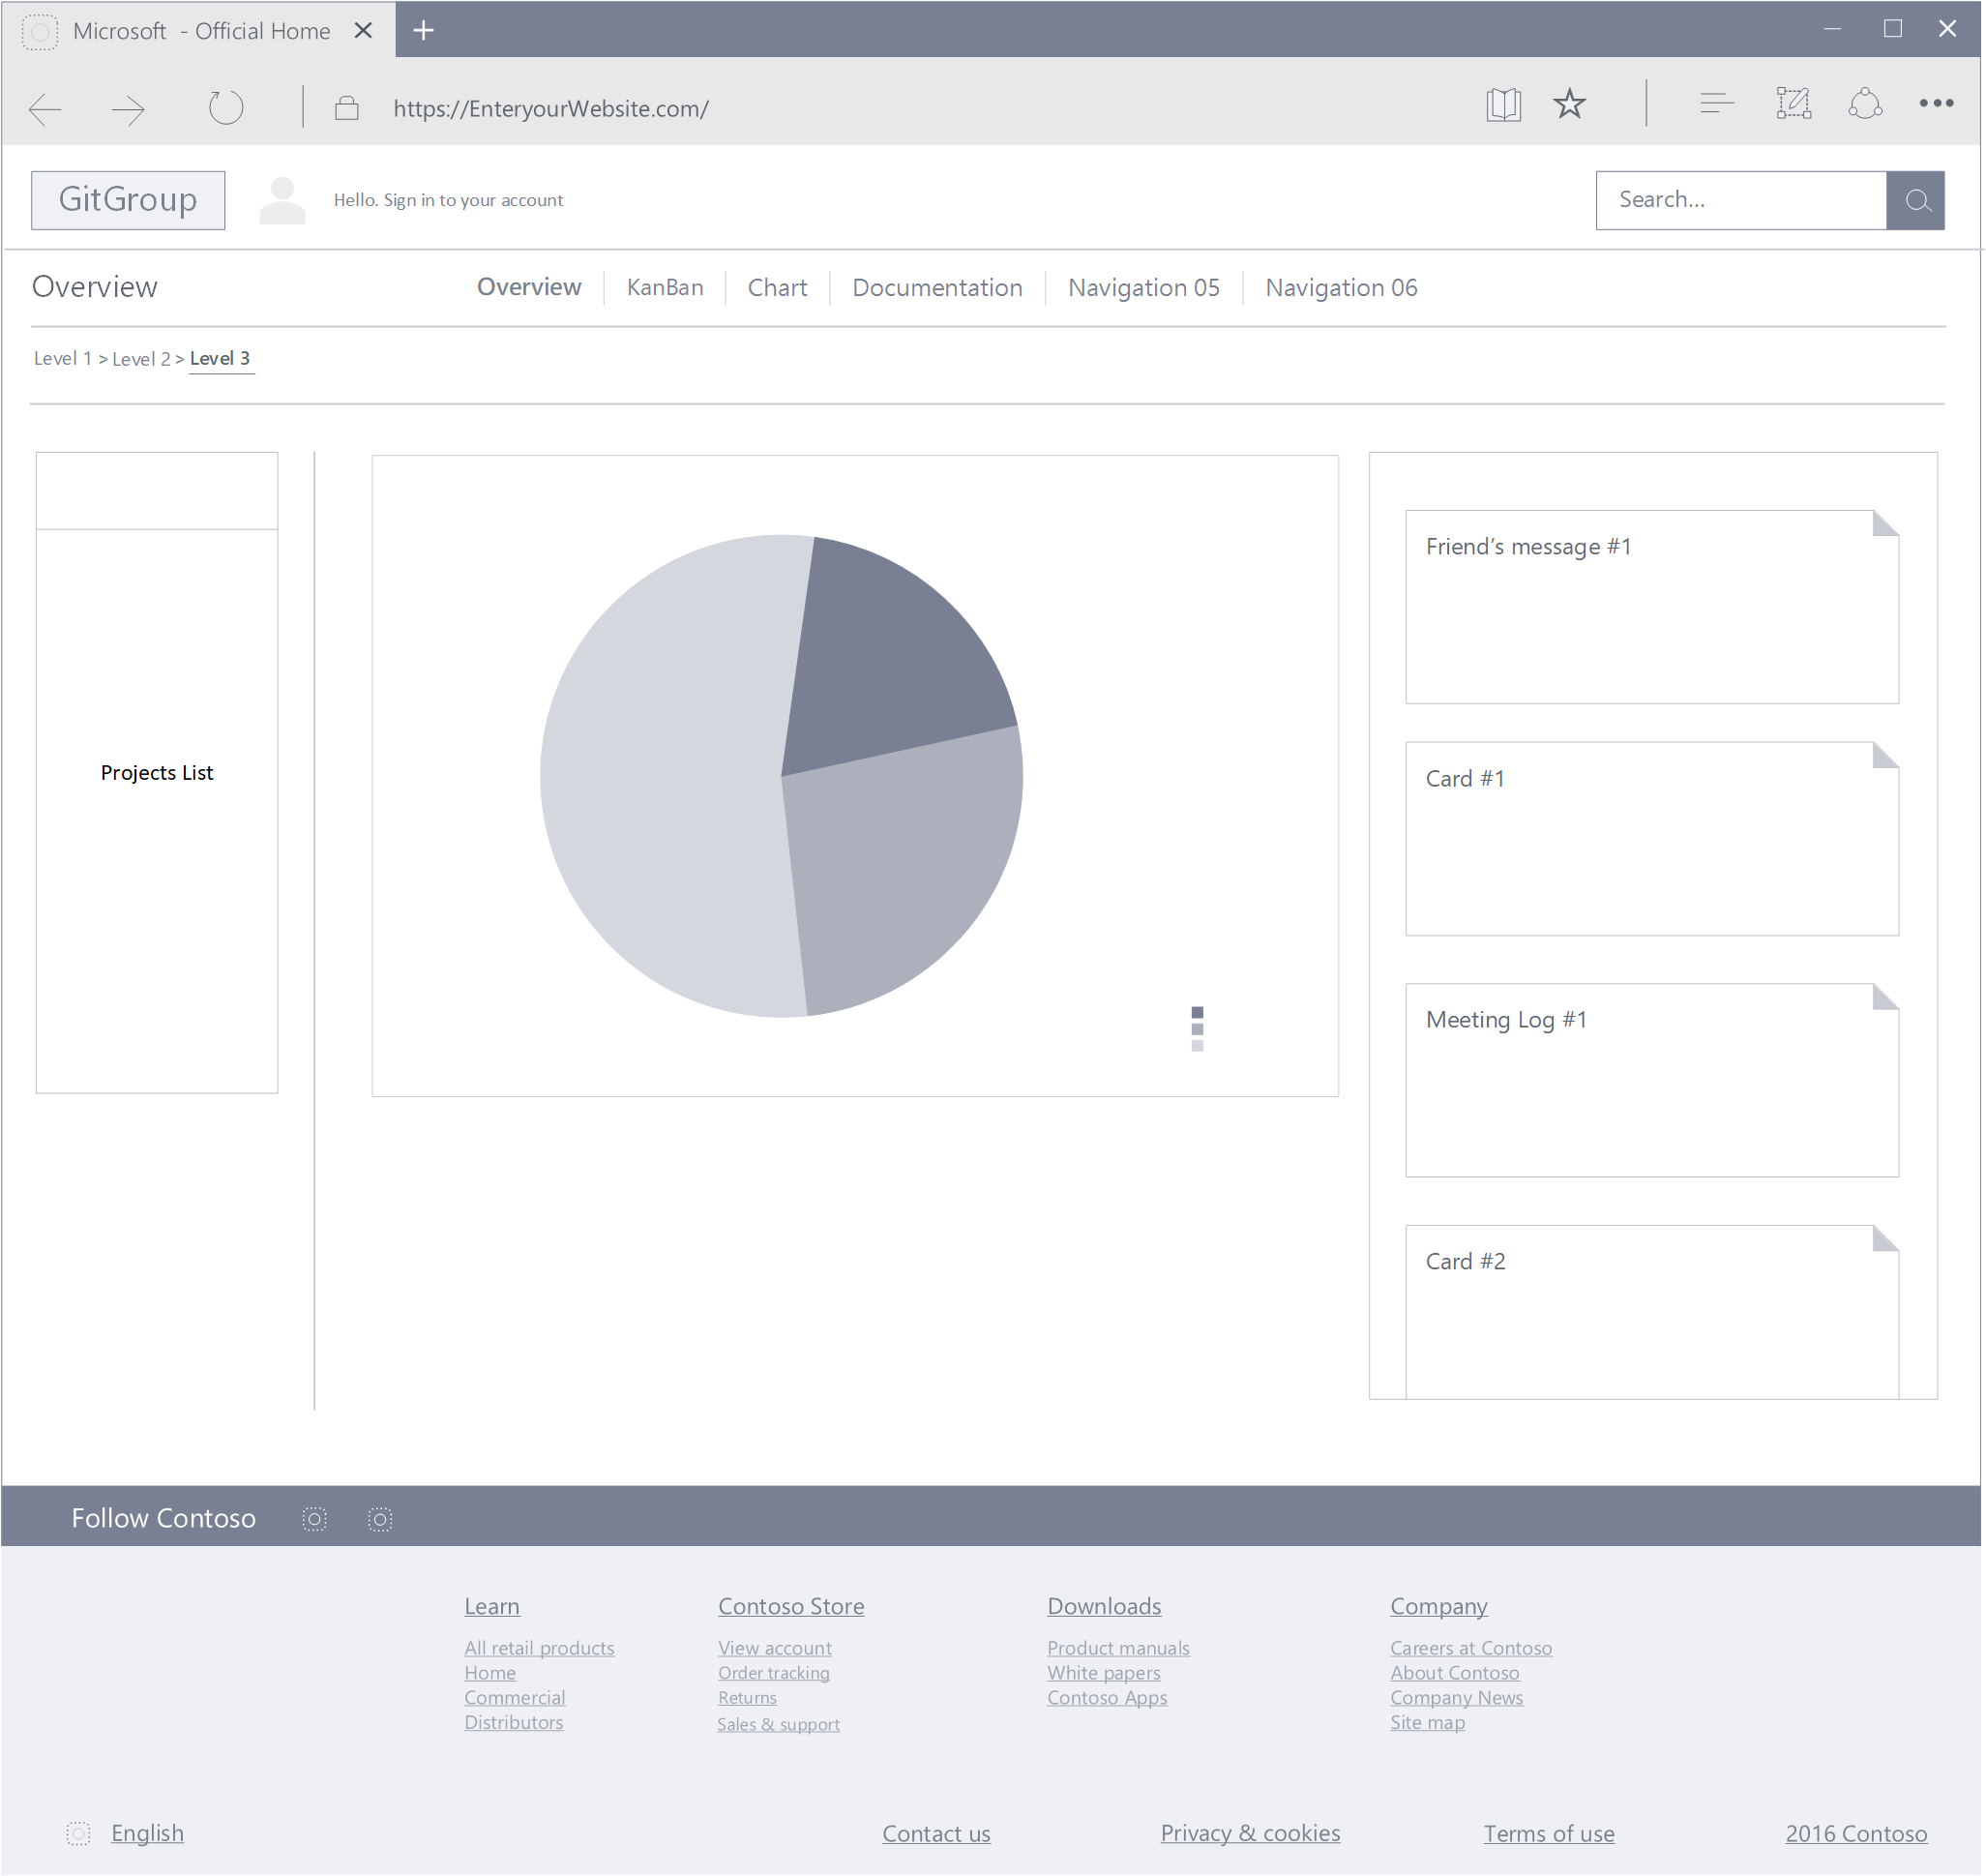
\includegraphics[width=0.6\textwidth]{./pics/OverviewInterface.png}
	\caption{Overview User Interface (Details in Appendix A)}
\end{figure}
\begin{figure}[H]
	\centering
	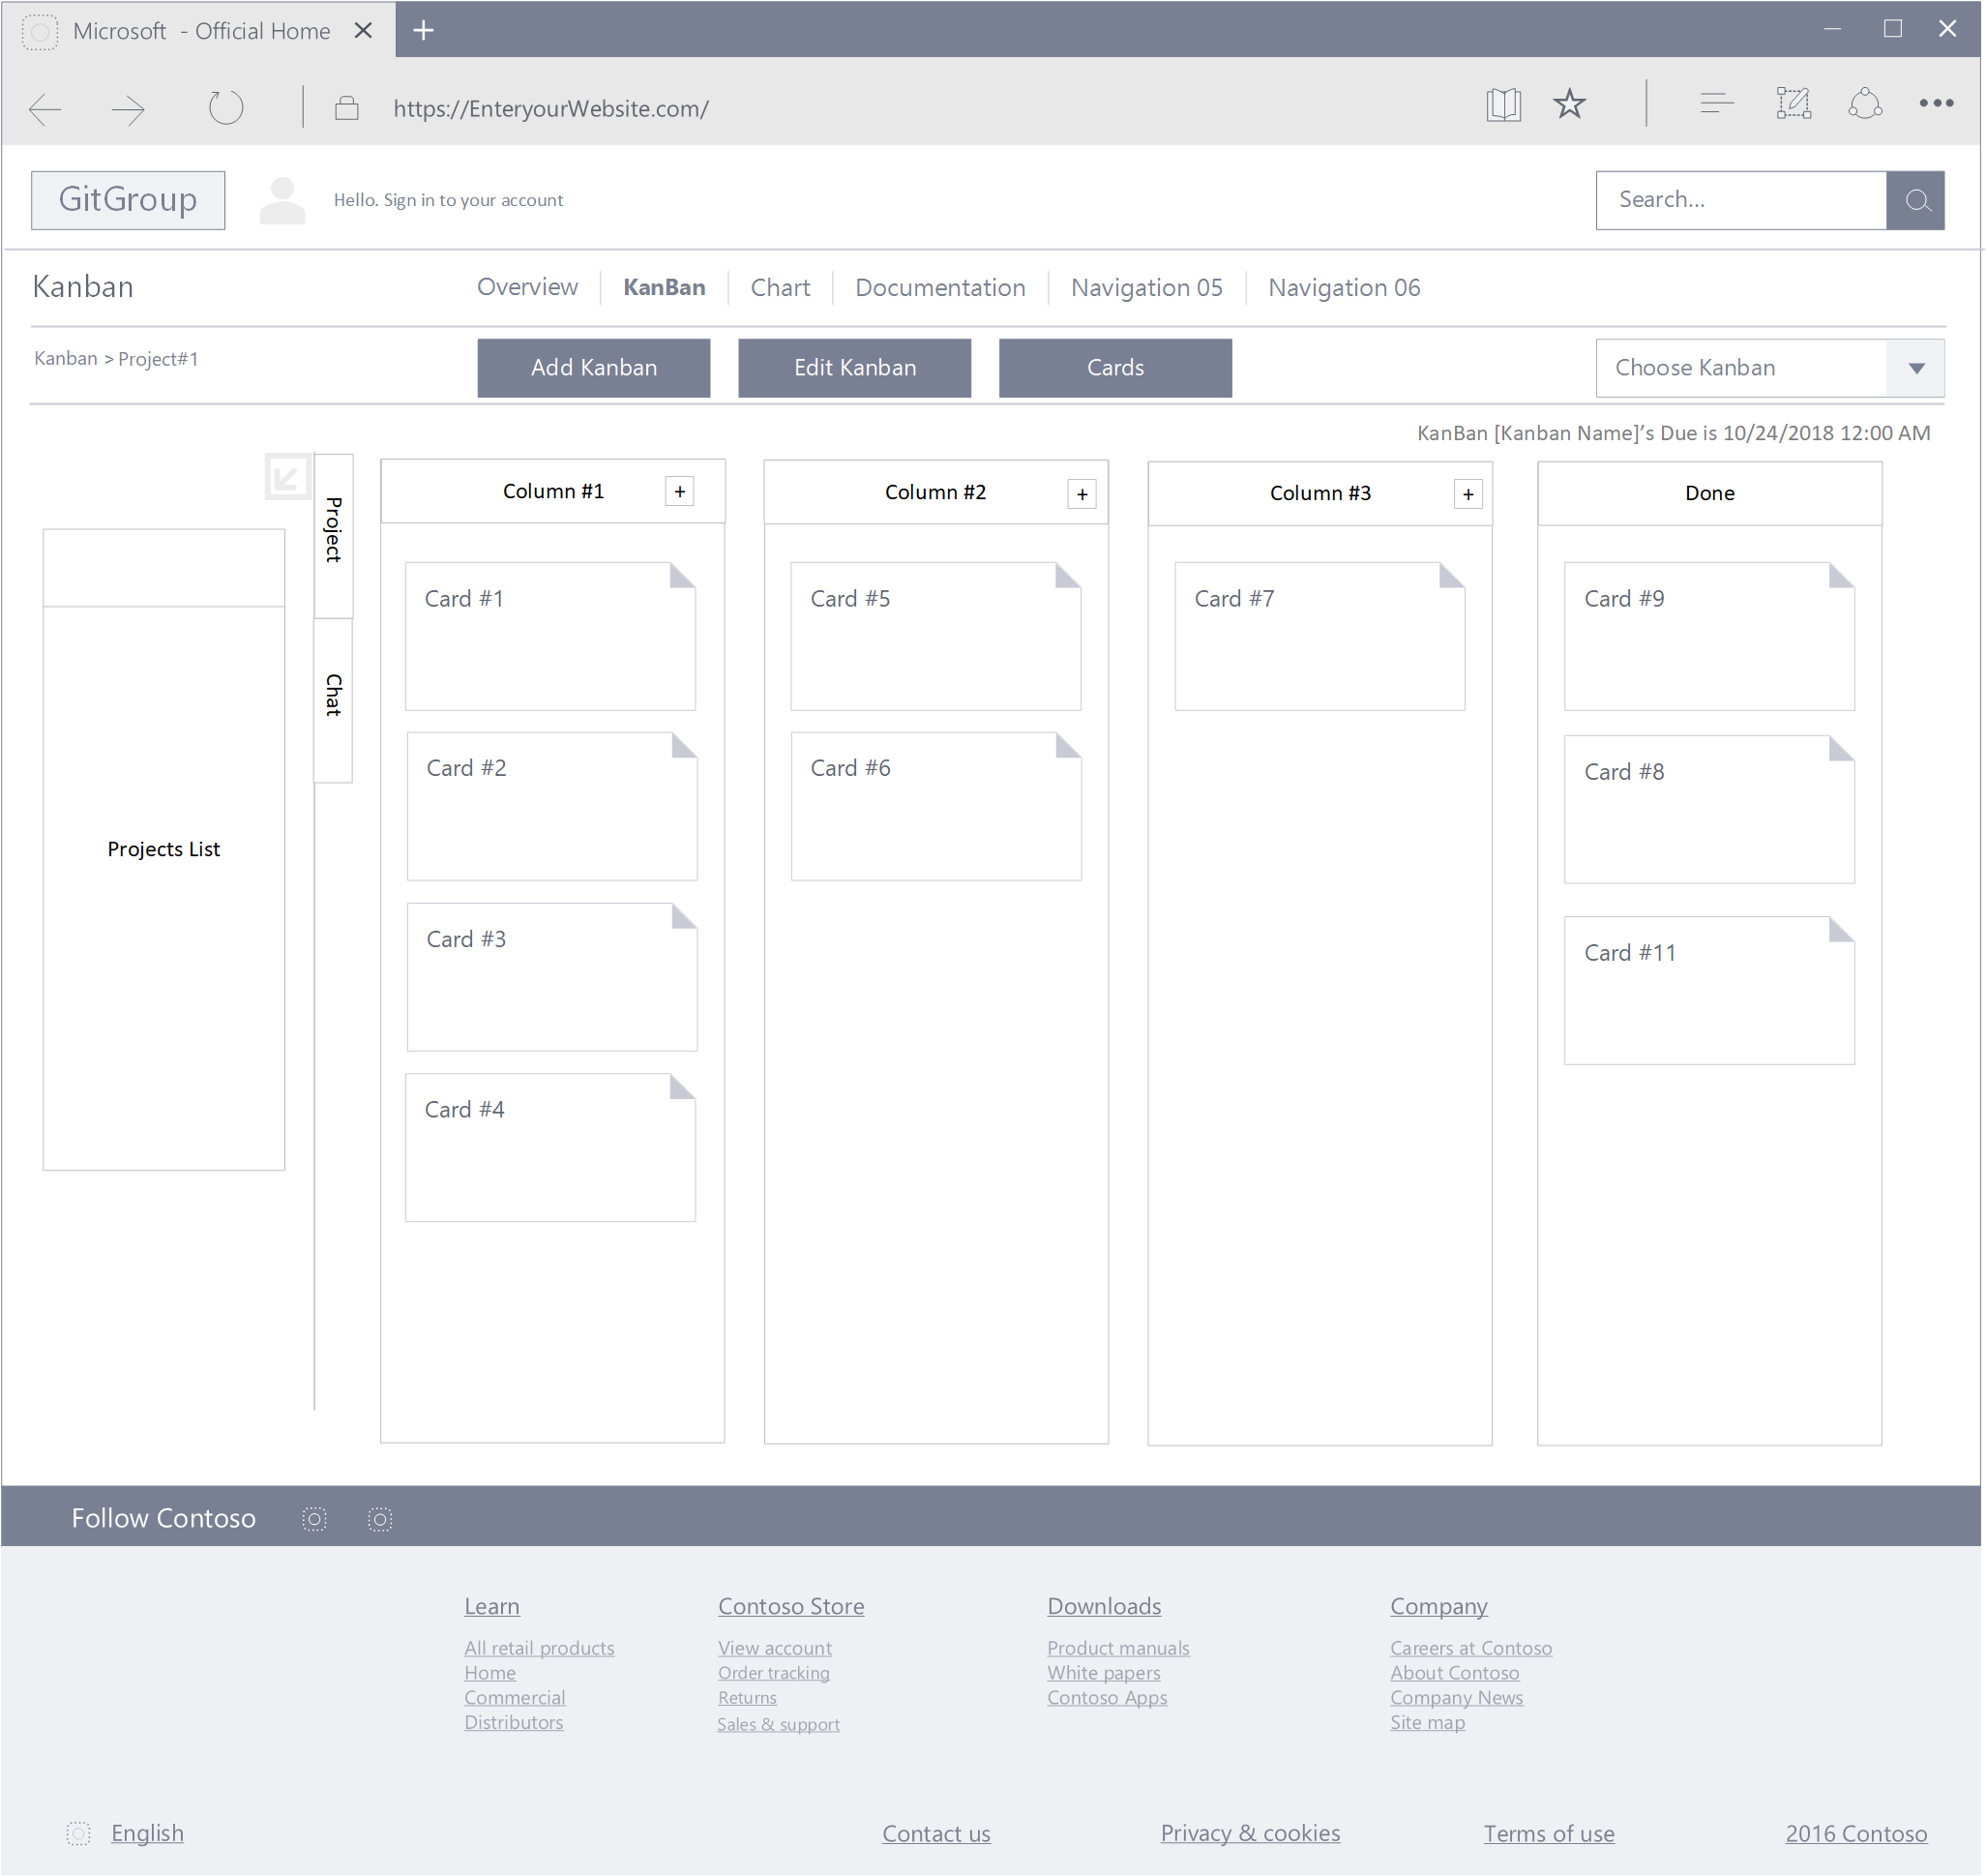
\includegraphics[width=0.6\textwidth]{./pics/KanbanInterface.png}
	\caption{KanBan User Interface (Details in Appendix A)}
\end{figure}
\begin{figure}[H]
	\centering
	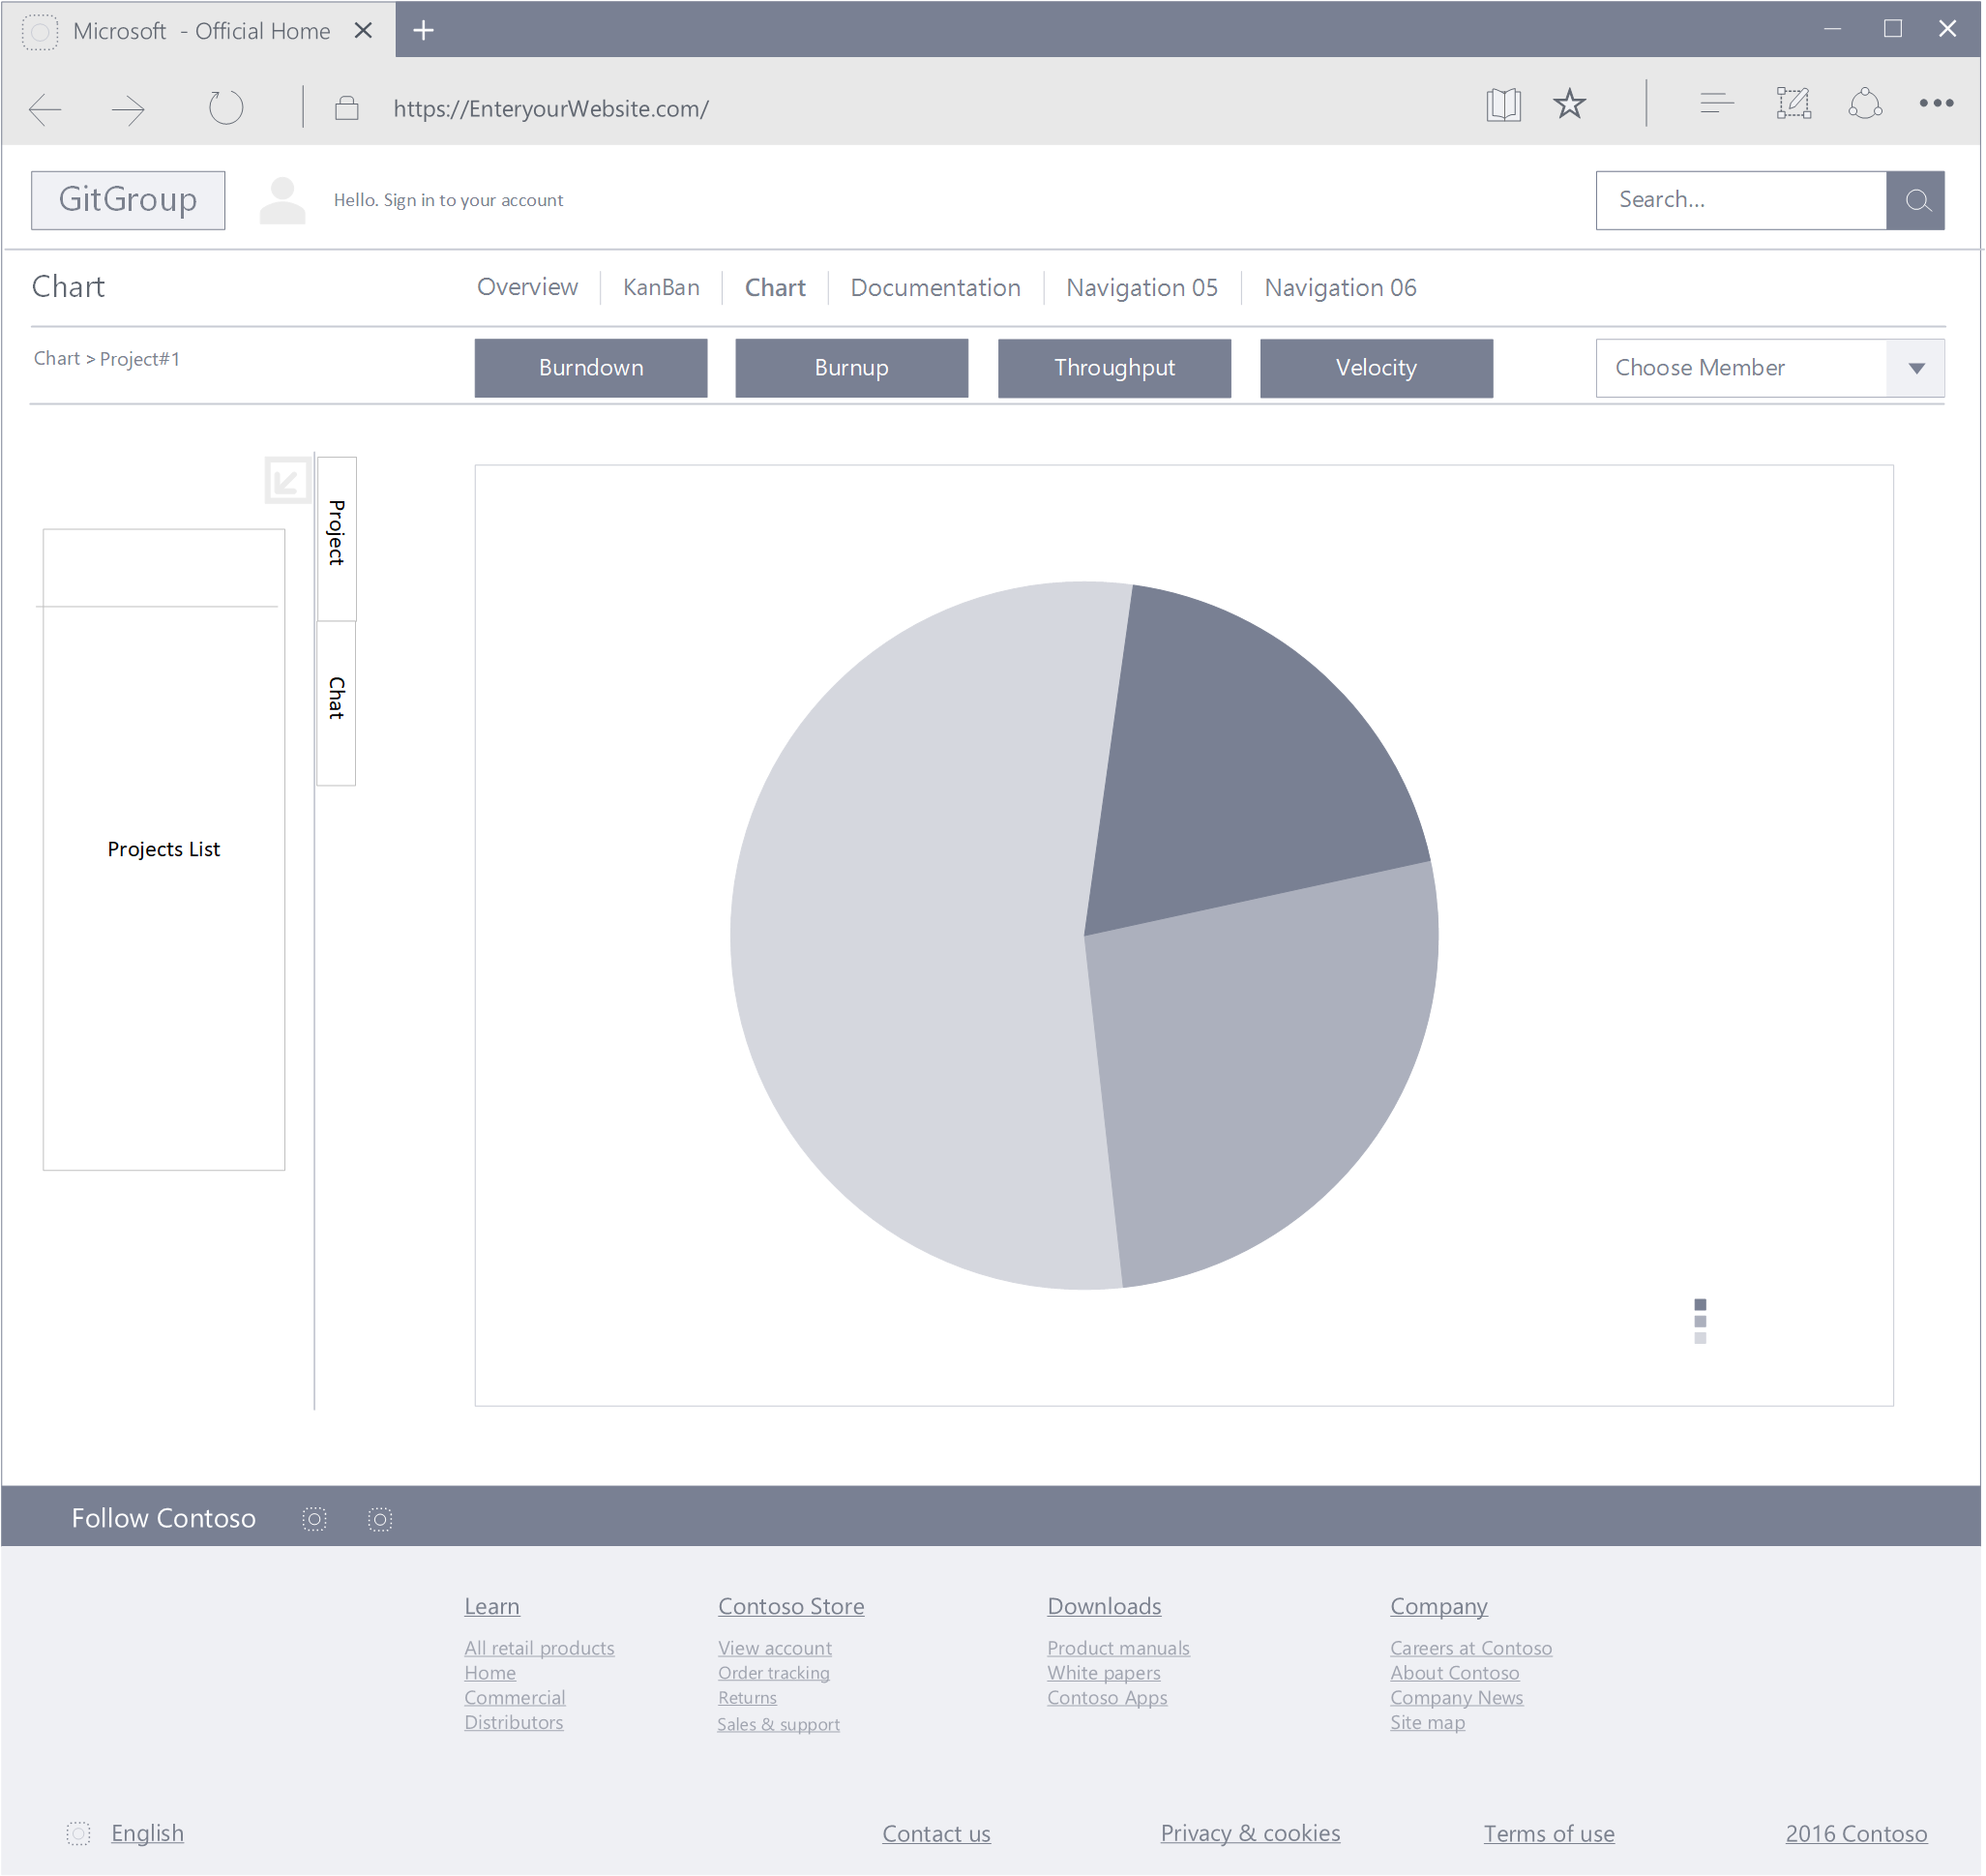
\includegraphics[width=0.6\textwidth]{./pics/ChartInterface.png}
	\caption{Chart User Interface (Details in Appendix A)}
\end{figure}
\section{Hardware Interfaces}
\section{Software Interfaces}
\section{Communication Interfaces}


% -----------------------------------------------------
% Chapter Requirements
% -----------------------------------------------------
\chapter{Requirements}
\section{User Requirements}
	\subsection{Functional User Requirement}
		\begin{enumerate}
			\renewcommand{\labelenumi}{{\textbf{\arabic{enumi}.}}}
			\item User shall be able to create a new project and new team in GitGroup.
			\item User shall be able to manage GitHub repositories and team members like add or remove repositories and members.
			\item User shall be able to use Kanban board to organize issues by dragging issue cards among several columns representing different stage of the development processes.
			\item User shall be able to analysis the development duration, quality and the team work situation of the project by using a variety of agile charts and analytics.
			also manage tasks like suggesting a new idea or tracking a bug. 
			\item User shall be able to organize an online meeting group chat, schedule and record the conference within the team or the global scope.
		\end{enumerate}
	\subsection{Non-Functional User Requirement}
		\begin{enumerate}
			\renewcommand{\labelenumi}{{\textbf{\arabic{enumi}.}}}
			\item The application shall be able to make GitHub easy to use, especially friendly for the person who has little development experience such as product manager.
			\item The application shall be quickly restored to operational status after a failure occurs.
			\item The app shall be reliable to uses with no downtime.
			\item The application shall be able to provide maximum security against malicious attack.
		\end{enumerate}
\section{System Requirements}
	\subsection{Functional System Requirement}
		\begin{enumerate}
			\item[\textbf{1.1}] Developers can create a new project and make a team with other developers.
			\item[\textbf{1.2}] Developers can remove a project and collaborators of the project after checking if the project is empty.
			\item[\textbf{2.1}] Developers can manage their team by inviting to or removing collaborators from their projects.
			\item[\textbf{2.2}] Developers can manage their repositories by adding or removing repositories of their projects.
			\item[\textbf{3.1}] Developers can classify issues by different stages of development process via putting them in different columns of Kanban board. 
			\item[\textbf{3.2}] Developers can add or remove a Kanban from their Kanban board.
			\item[\textbf{3.3}] Developers can customize their own stage by editing column name except Done column.
			\item[\textbf{3.4}]	Developers can close issues by dragging it to the Done column, which will automatically close issues in the GitHub. 
			\item[\textbf{4.1}] Project manager can track and communicate the progress of their projects by burn down and burn up charts.
			\item[\textbf{4.2}] Project manager can measure how much work a team can used in eXtreme Programming and Scrum from throughput chart.
			\item[\textbf{4.3}] Project manager can analysis the velocity of project going from velocity chart.
			\item[\textbf{5.1}] Team leader can organize an online meeting group chat within their team.
			\item[\textbf{5.2}] Developers can organize an online meeting group chat within the global.
			\item[\textbf{5.3}] Developers can receive a meeting notification from team leader.
			\item[\textbf{5.4}] Developers can set an alarm for notifying the coming events on a conference schedule form.
			\item[\textbf{5.5}] Developers shall be able to record content of meeting on a meeting notebook.
		\end{enumerate}
	\subsection{Non-Functional System Requirement}
		\begin{enumerate}
			\item[\textbf{1.1}] The user shall be able to use all the app functions without any kind of training. The average number of questions call about how to use app shall not exceed 10 per day.
			\item[\textbf{1.2}] The app shall be available for any kind of mobile device and PC.
			\item[\textbf{2.1}]
			\item[\textbf{3.1}] The app shall be available to all users during whole day (Mon-Sun, 00:00~00:00)
			\item[\textbf{4.1}] The app shall not expose contact information to other users. 
			\item[\textbf{4.2}] The app should minimize the amount of personally identifying information (PII) that it collects.
		\end{enumerate}
	

\chapter{System Models}
\section{Use Case Diagram}
\begin{figure}[H]
	\centering
	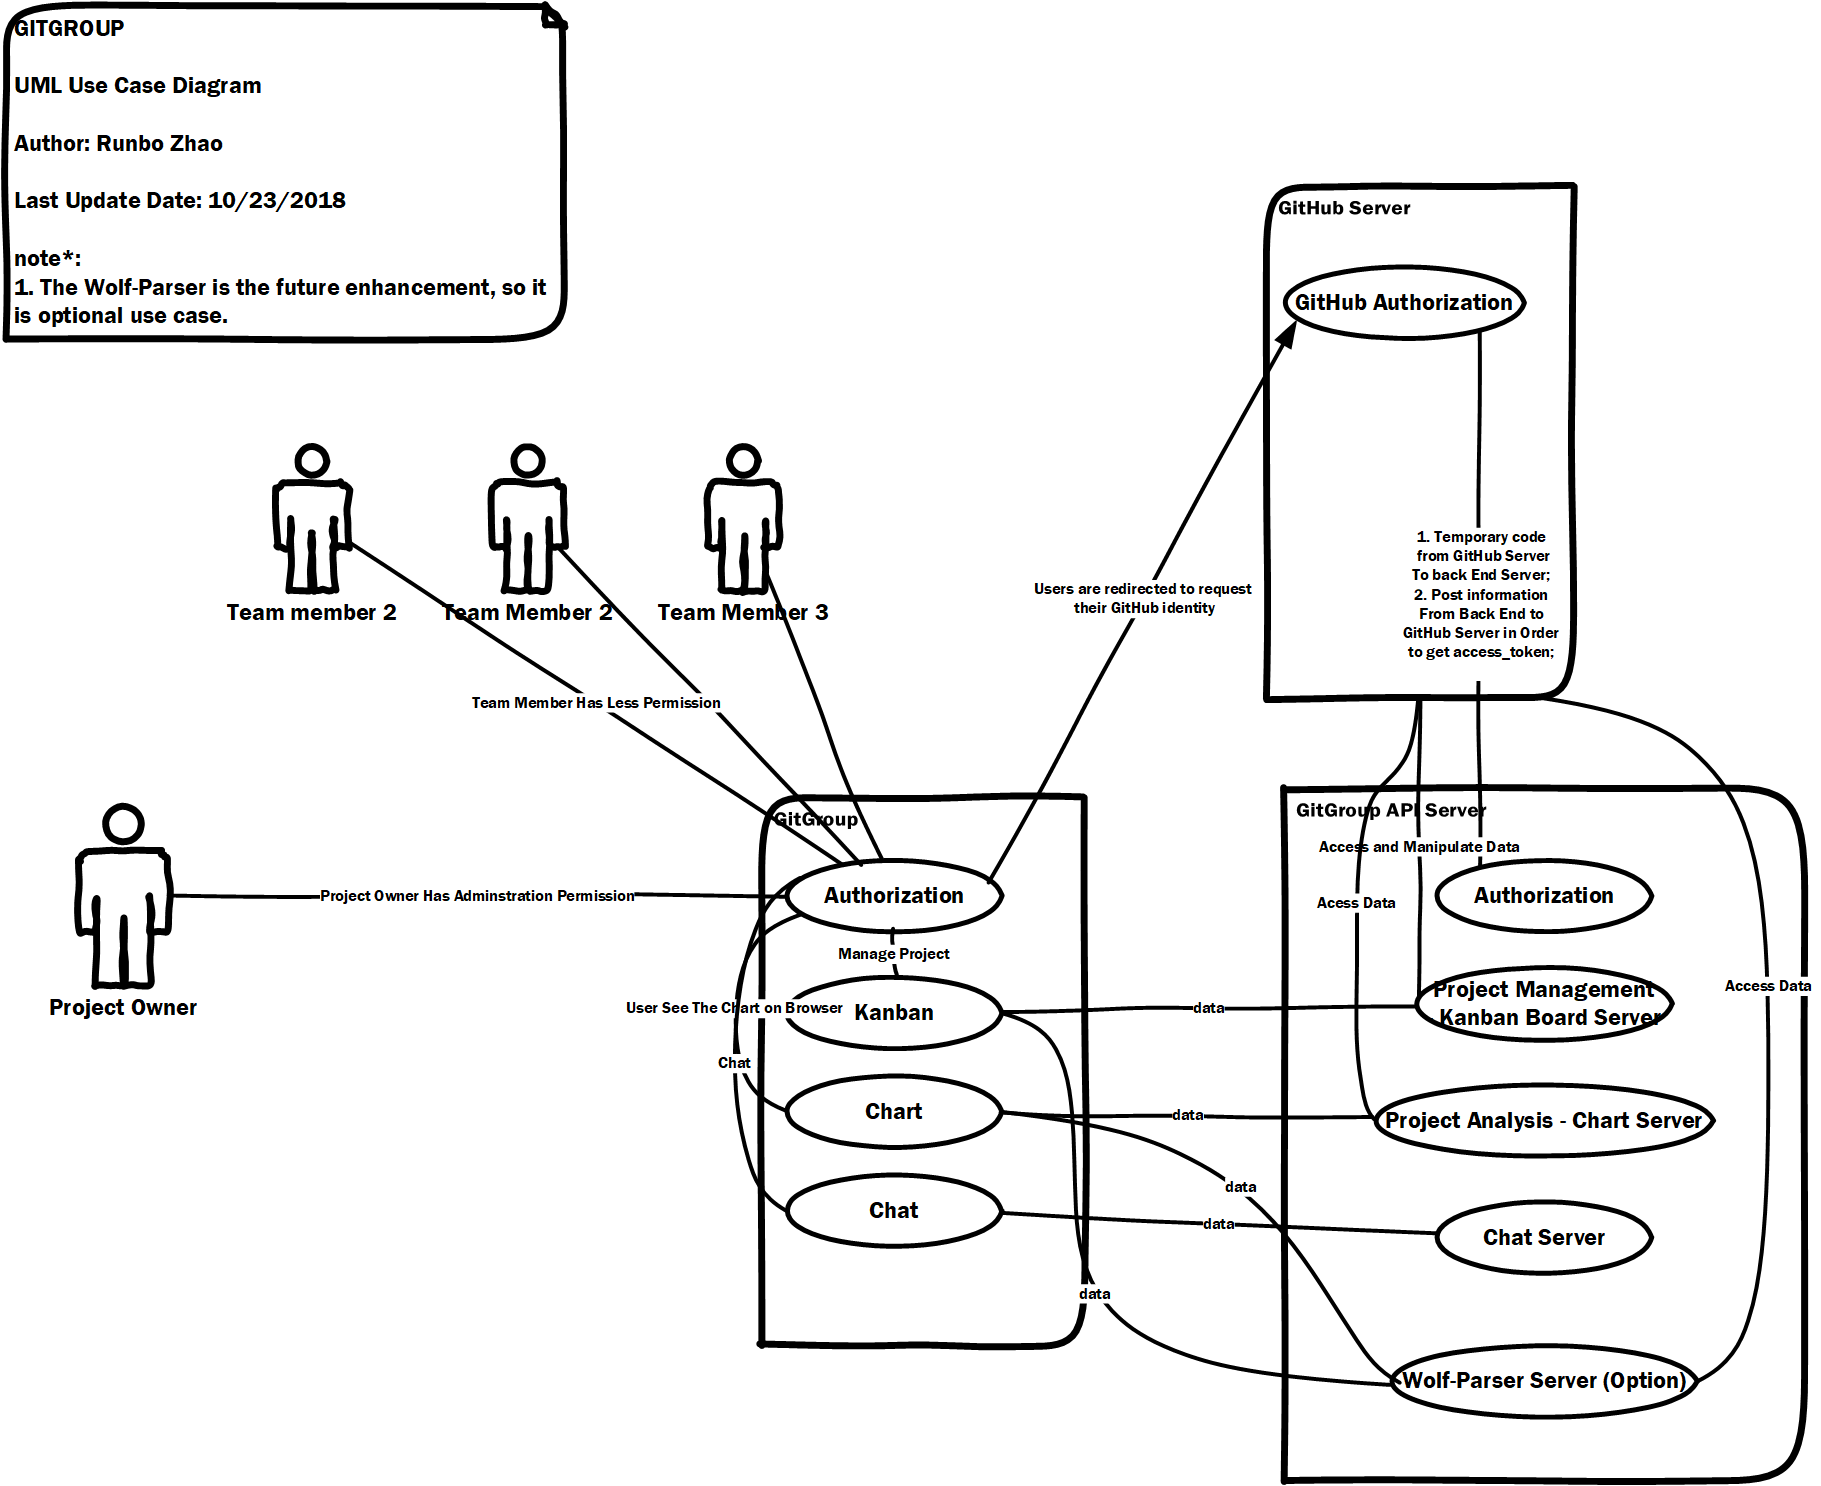
\includegraphics[width=0.7\textwidth]{./pics/UseCaseDiagram.png}
	\caption{Use Case Diagram (Details in Appendix A)}
\end{figure}
\section{Activity Diagram}
\begin{figure}[H]
	\centering
	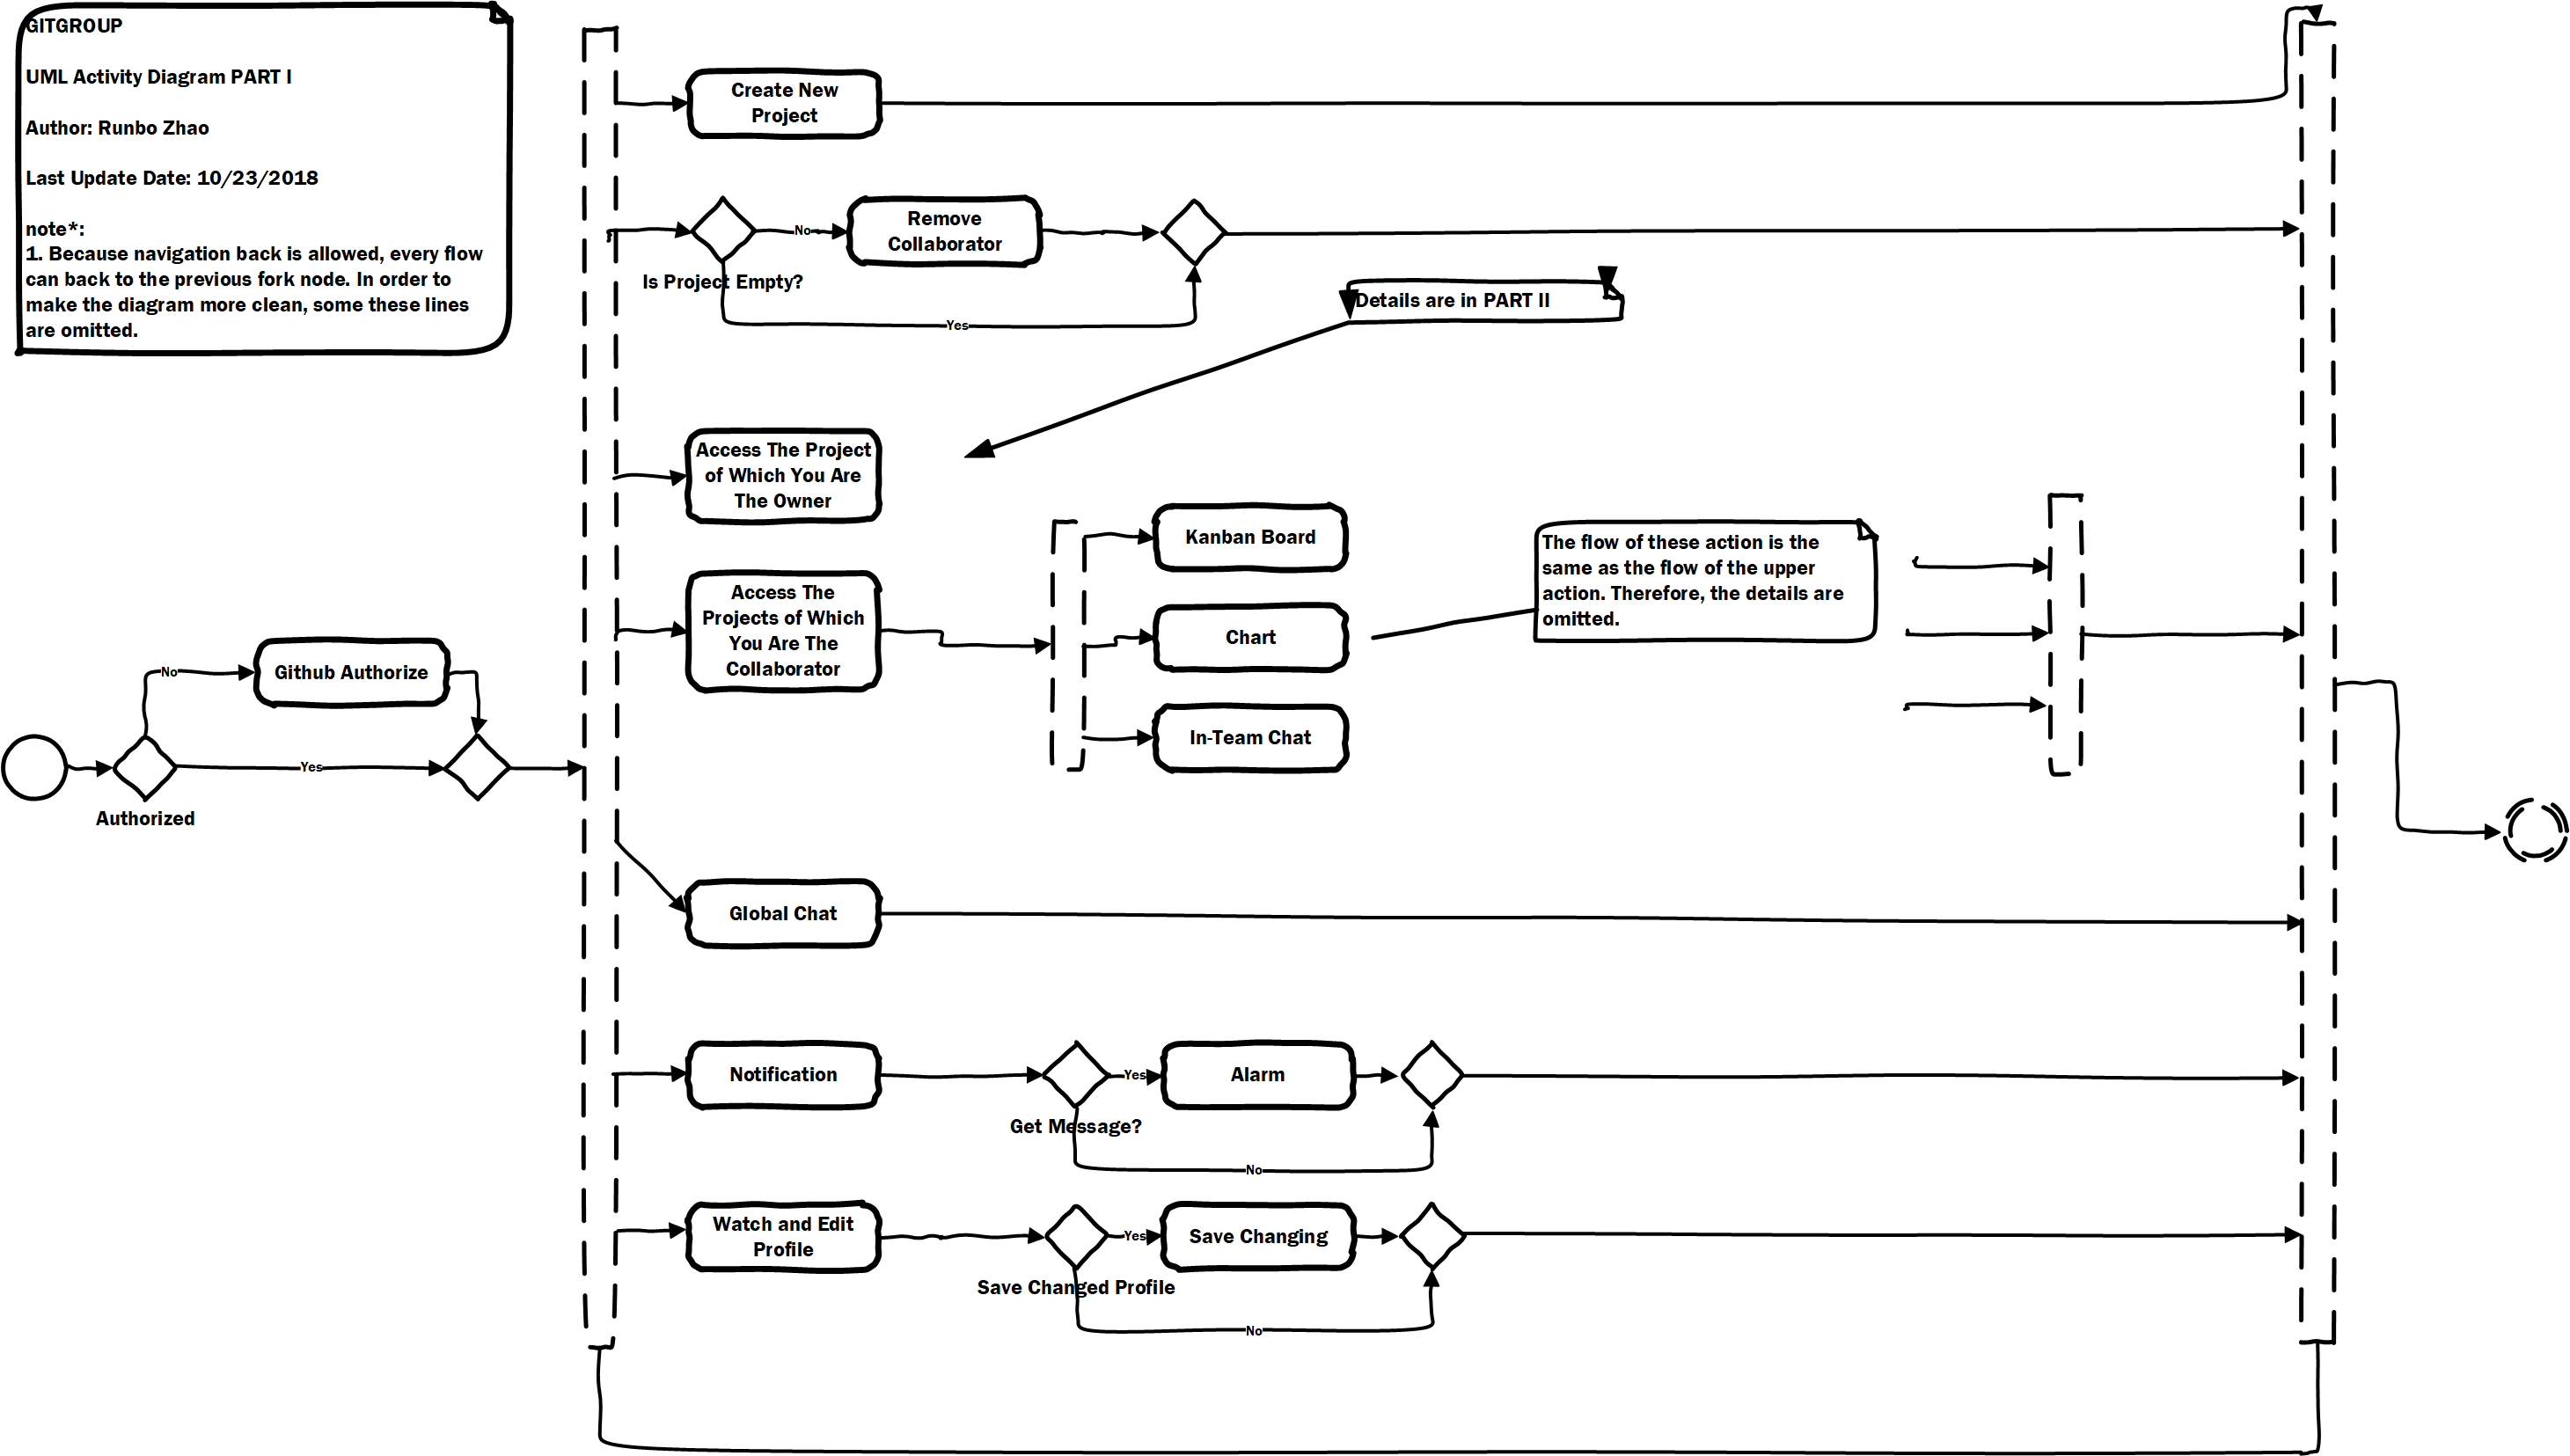
\includegraphics[width=0.7\textwidth]{./pics/ActivatyDiagramPARTI.png}
	\caption{Activity Diagram PART I (Details in Appendix A)}
\end{figure}
\begin{figure}[H]
	\centering
	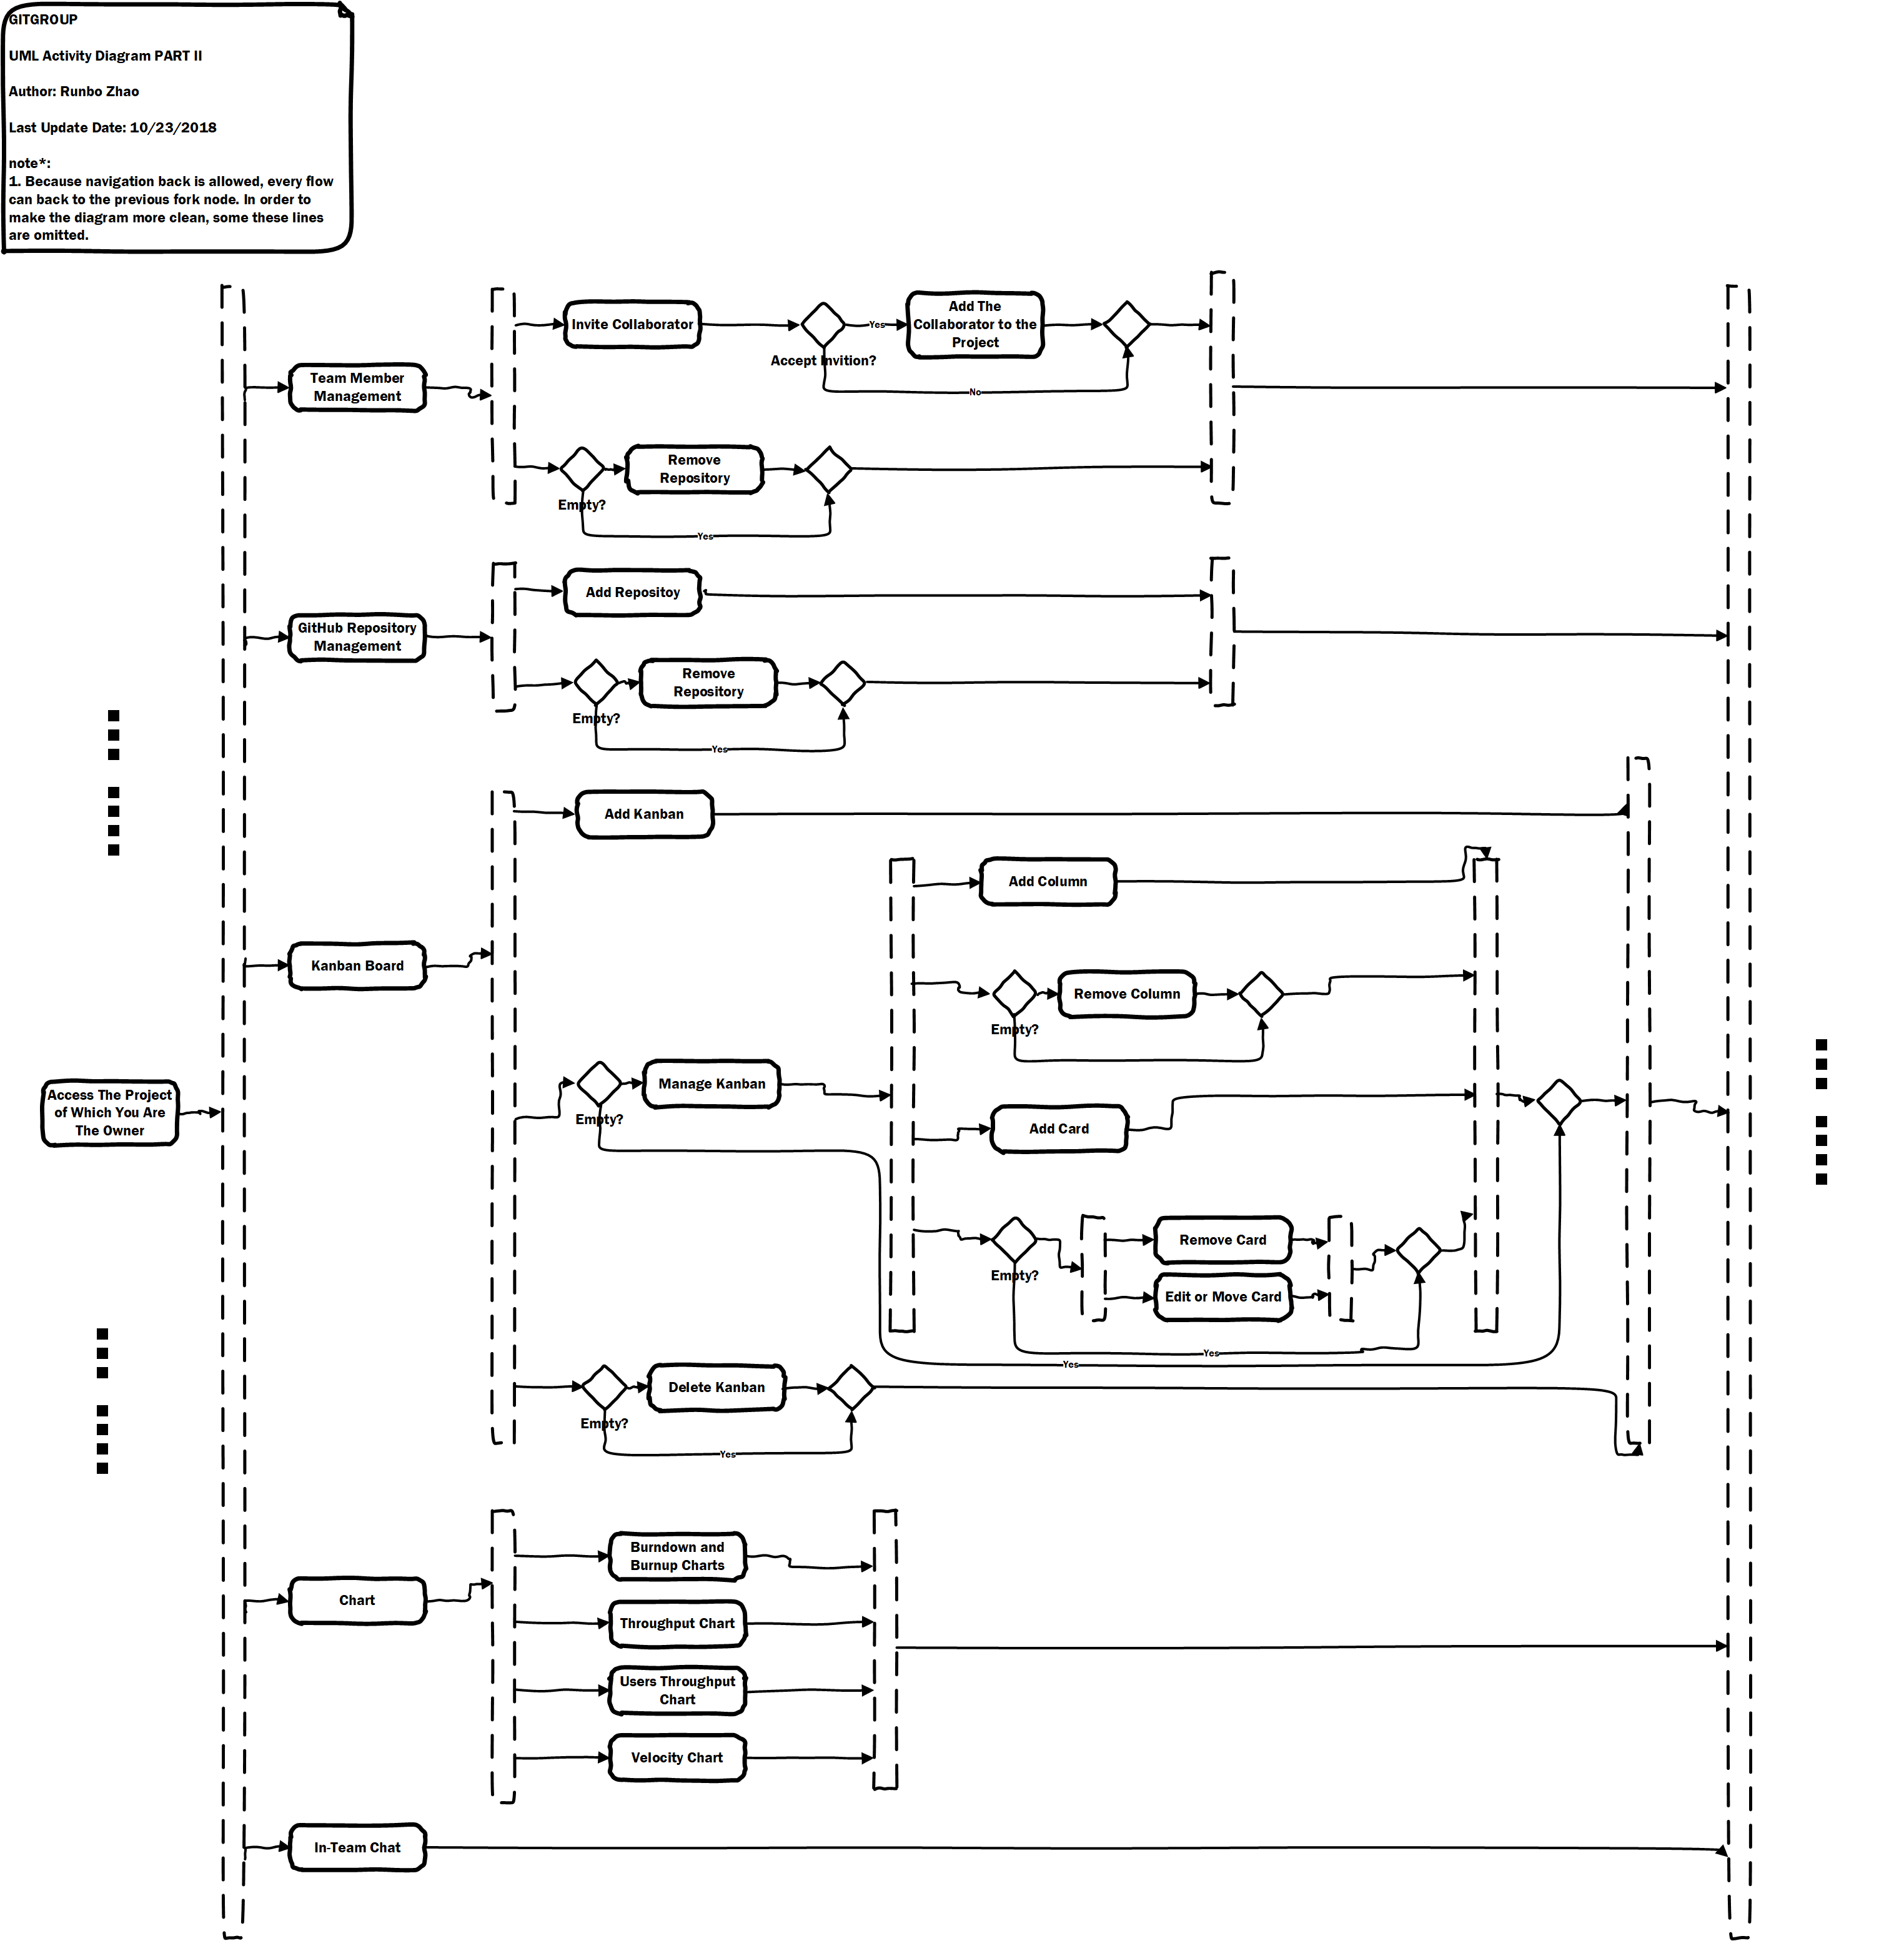
\includegraphics[width=0.7\textwidth]{./pics/ActivatyDiagramPARTII.png}
	\caption{Activity Diagram PART II (Details in Appendix A)}
\end{figure}
\section{Sequence Diagram}
\begin{figure}[H]
	\centering
	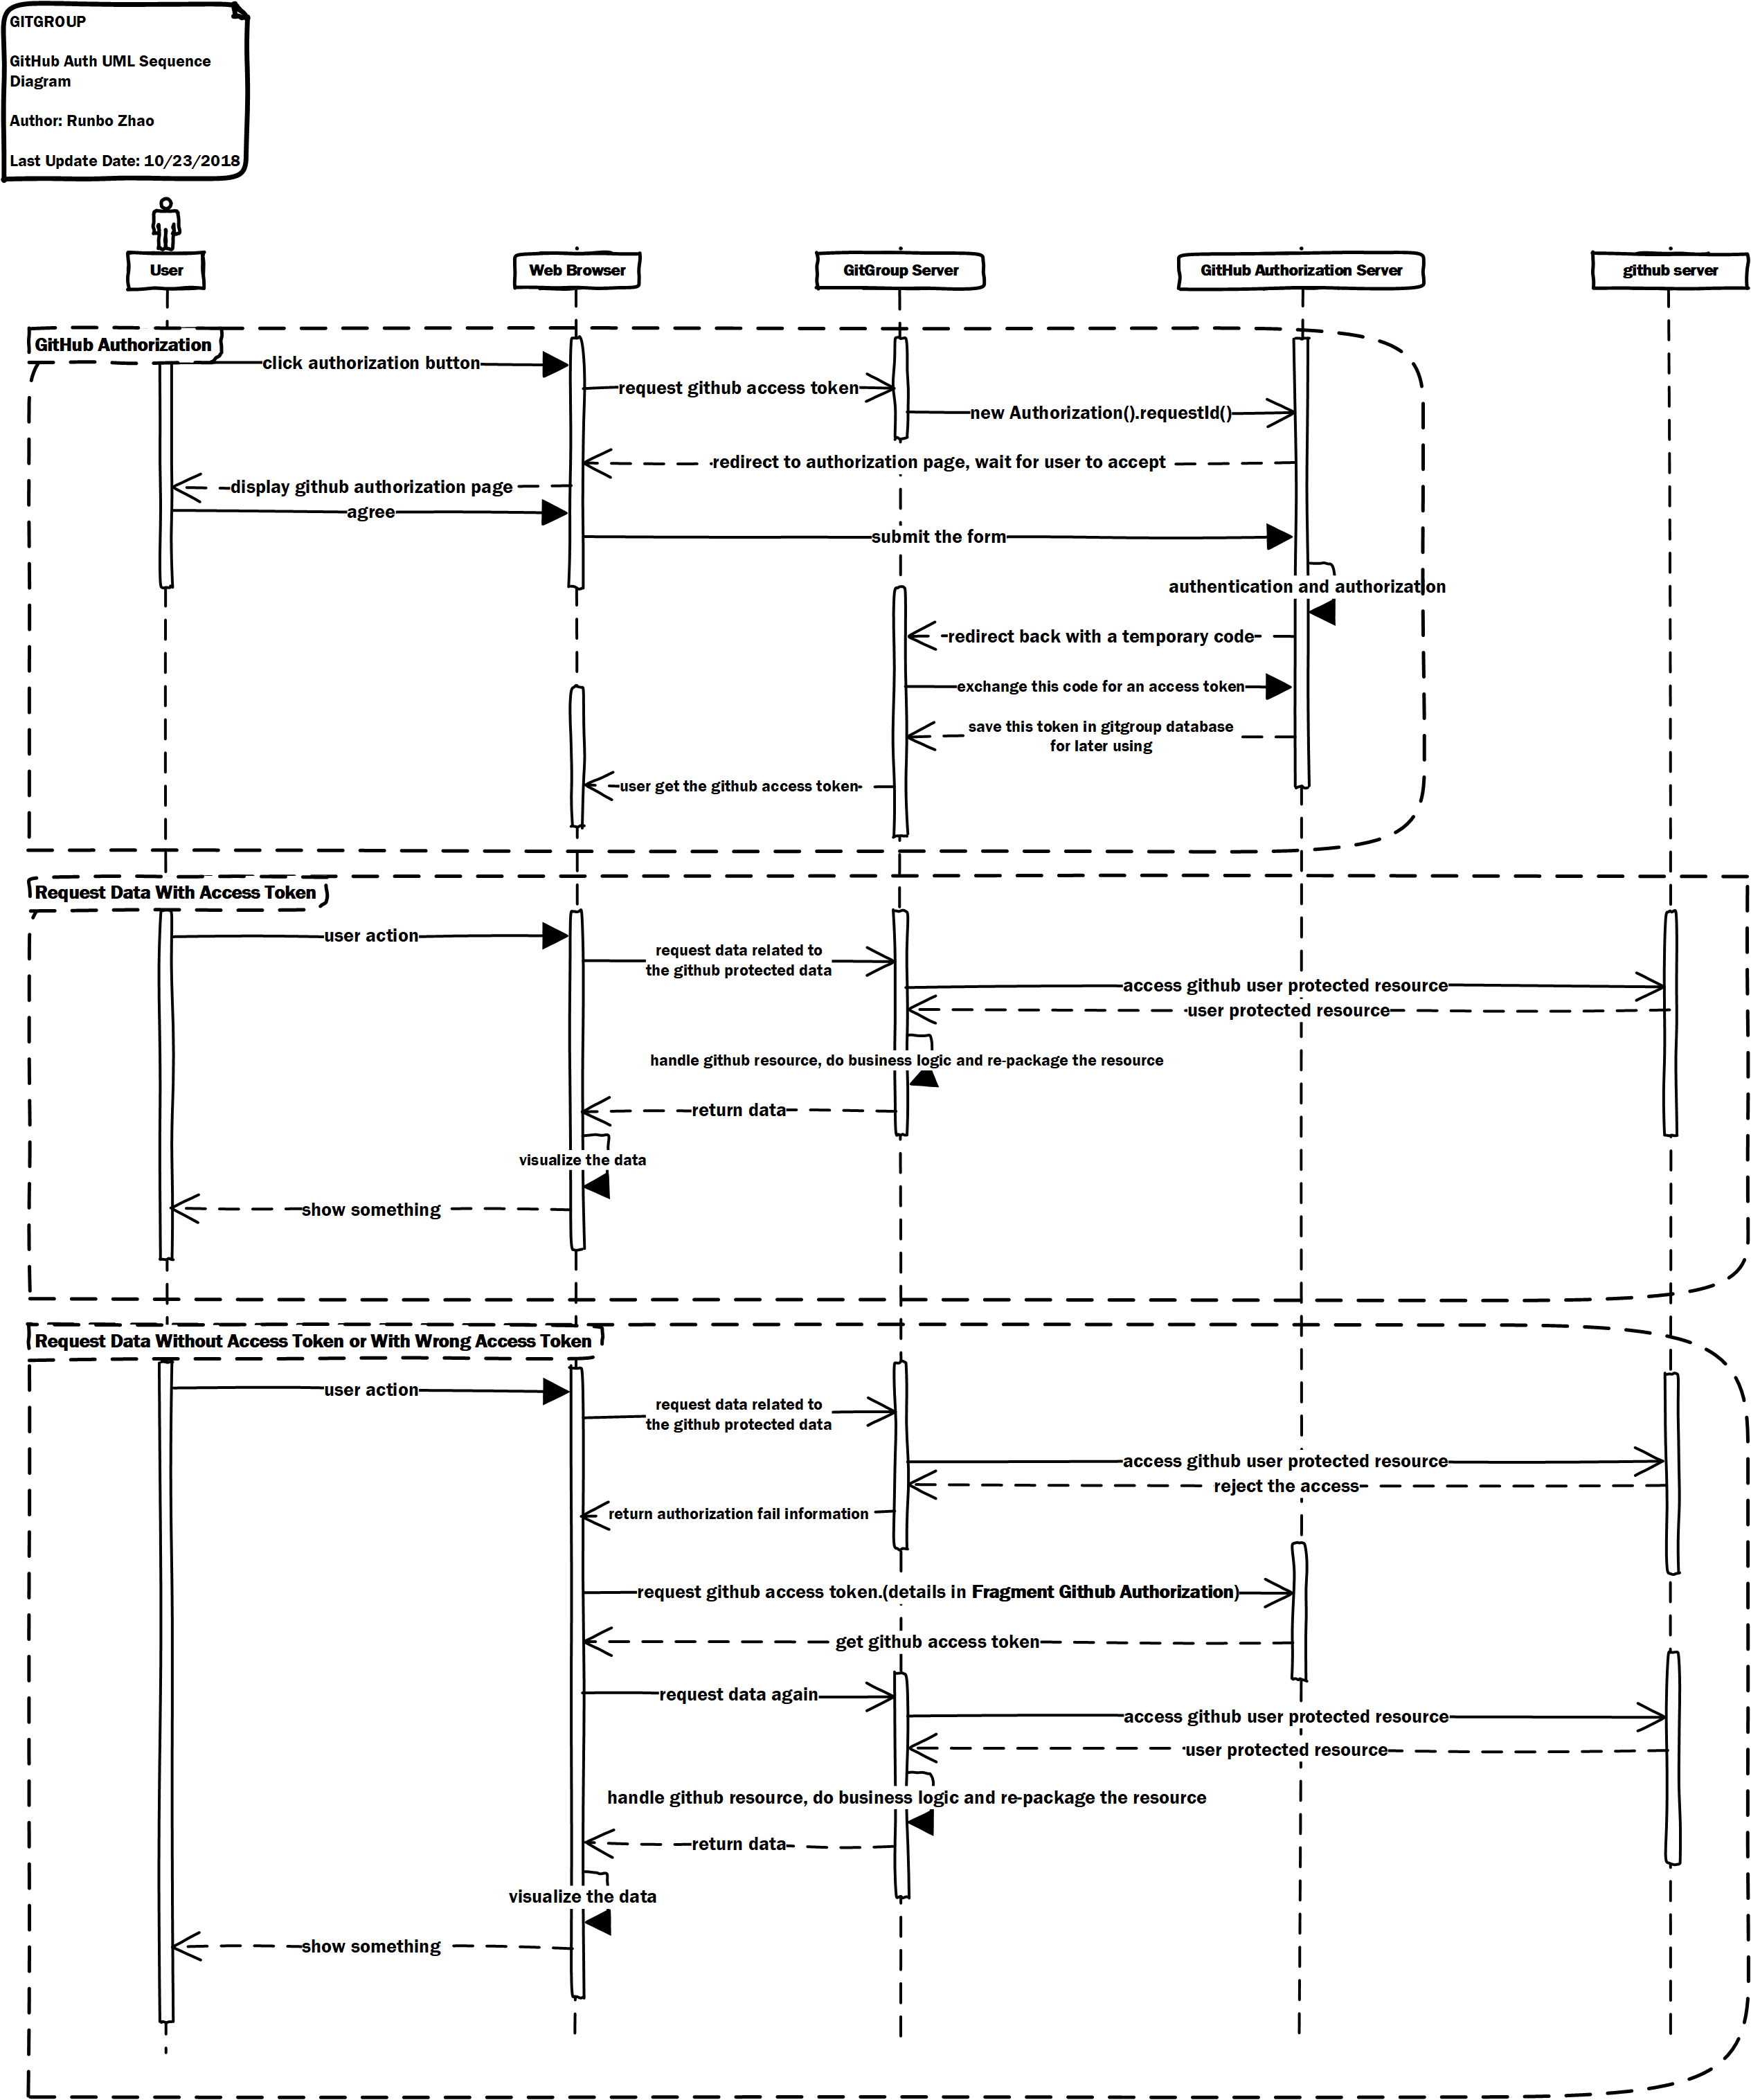
\includegraphics[width=0.7\textwidth]{./pics/AuthSequenceDiagram.png}
	\caption{Sequence Diagram For Authorization (Details in Appendix A)}
\end{figure}

\begin{figure}[H]
	\centering
	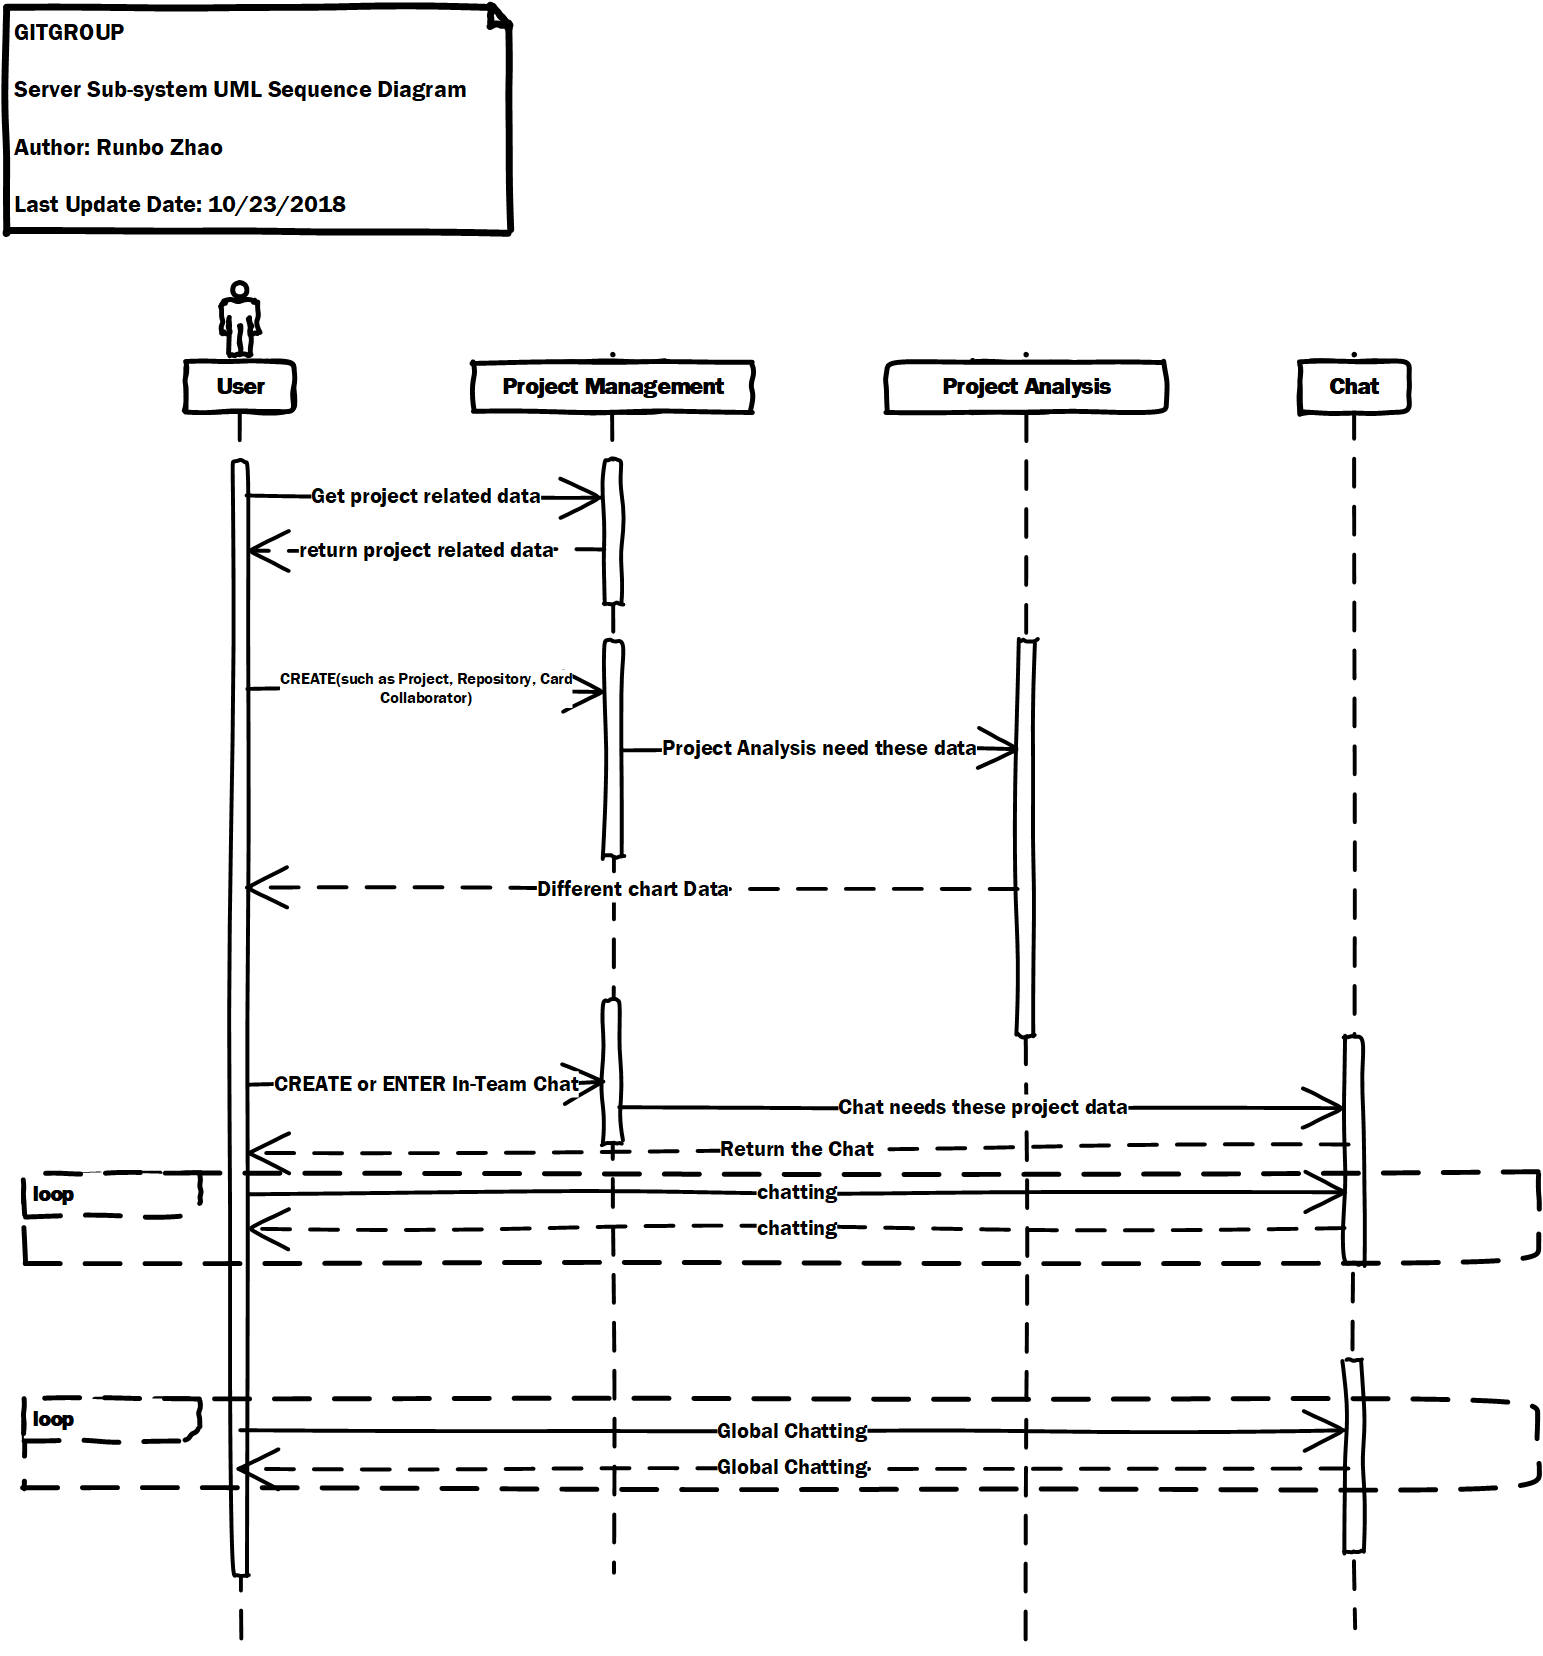
\includegraphics[width=0.7\textwidth]{./pics/SubSysSequenceDiagram.png}
	\caption{Sequence Diagram For Sub-Systems (Details in Appendix A)}
\end{figure}

\section{Class Diagram}
\begin{figure}[H]
	\centering
	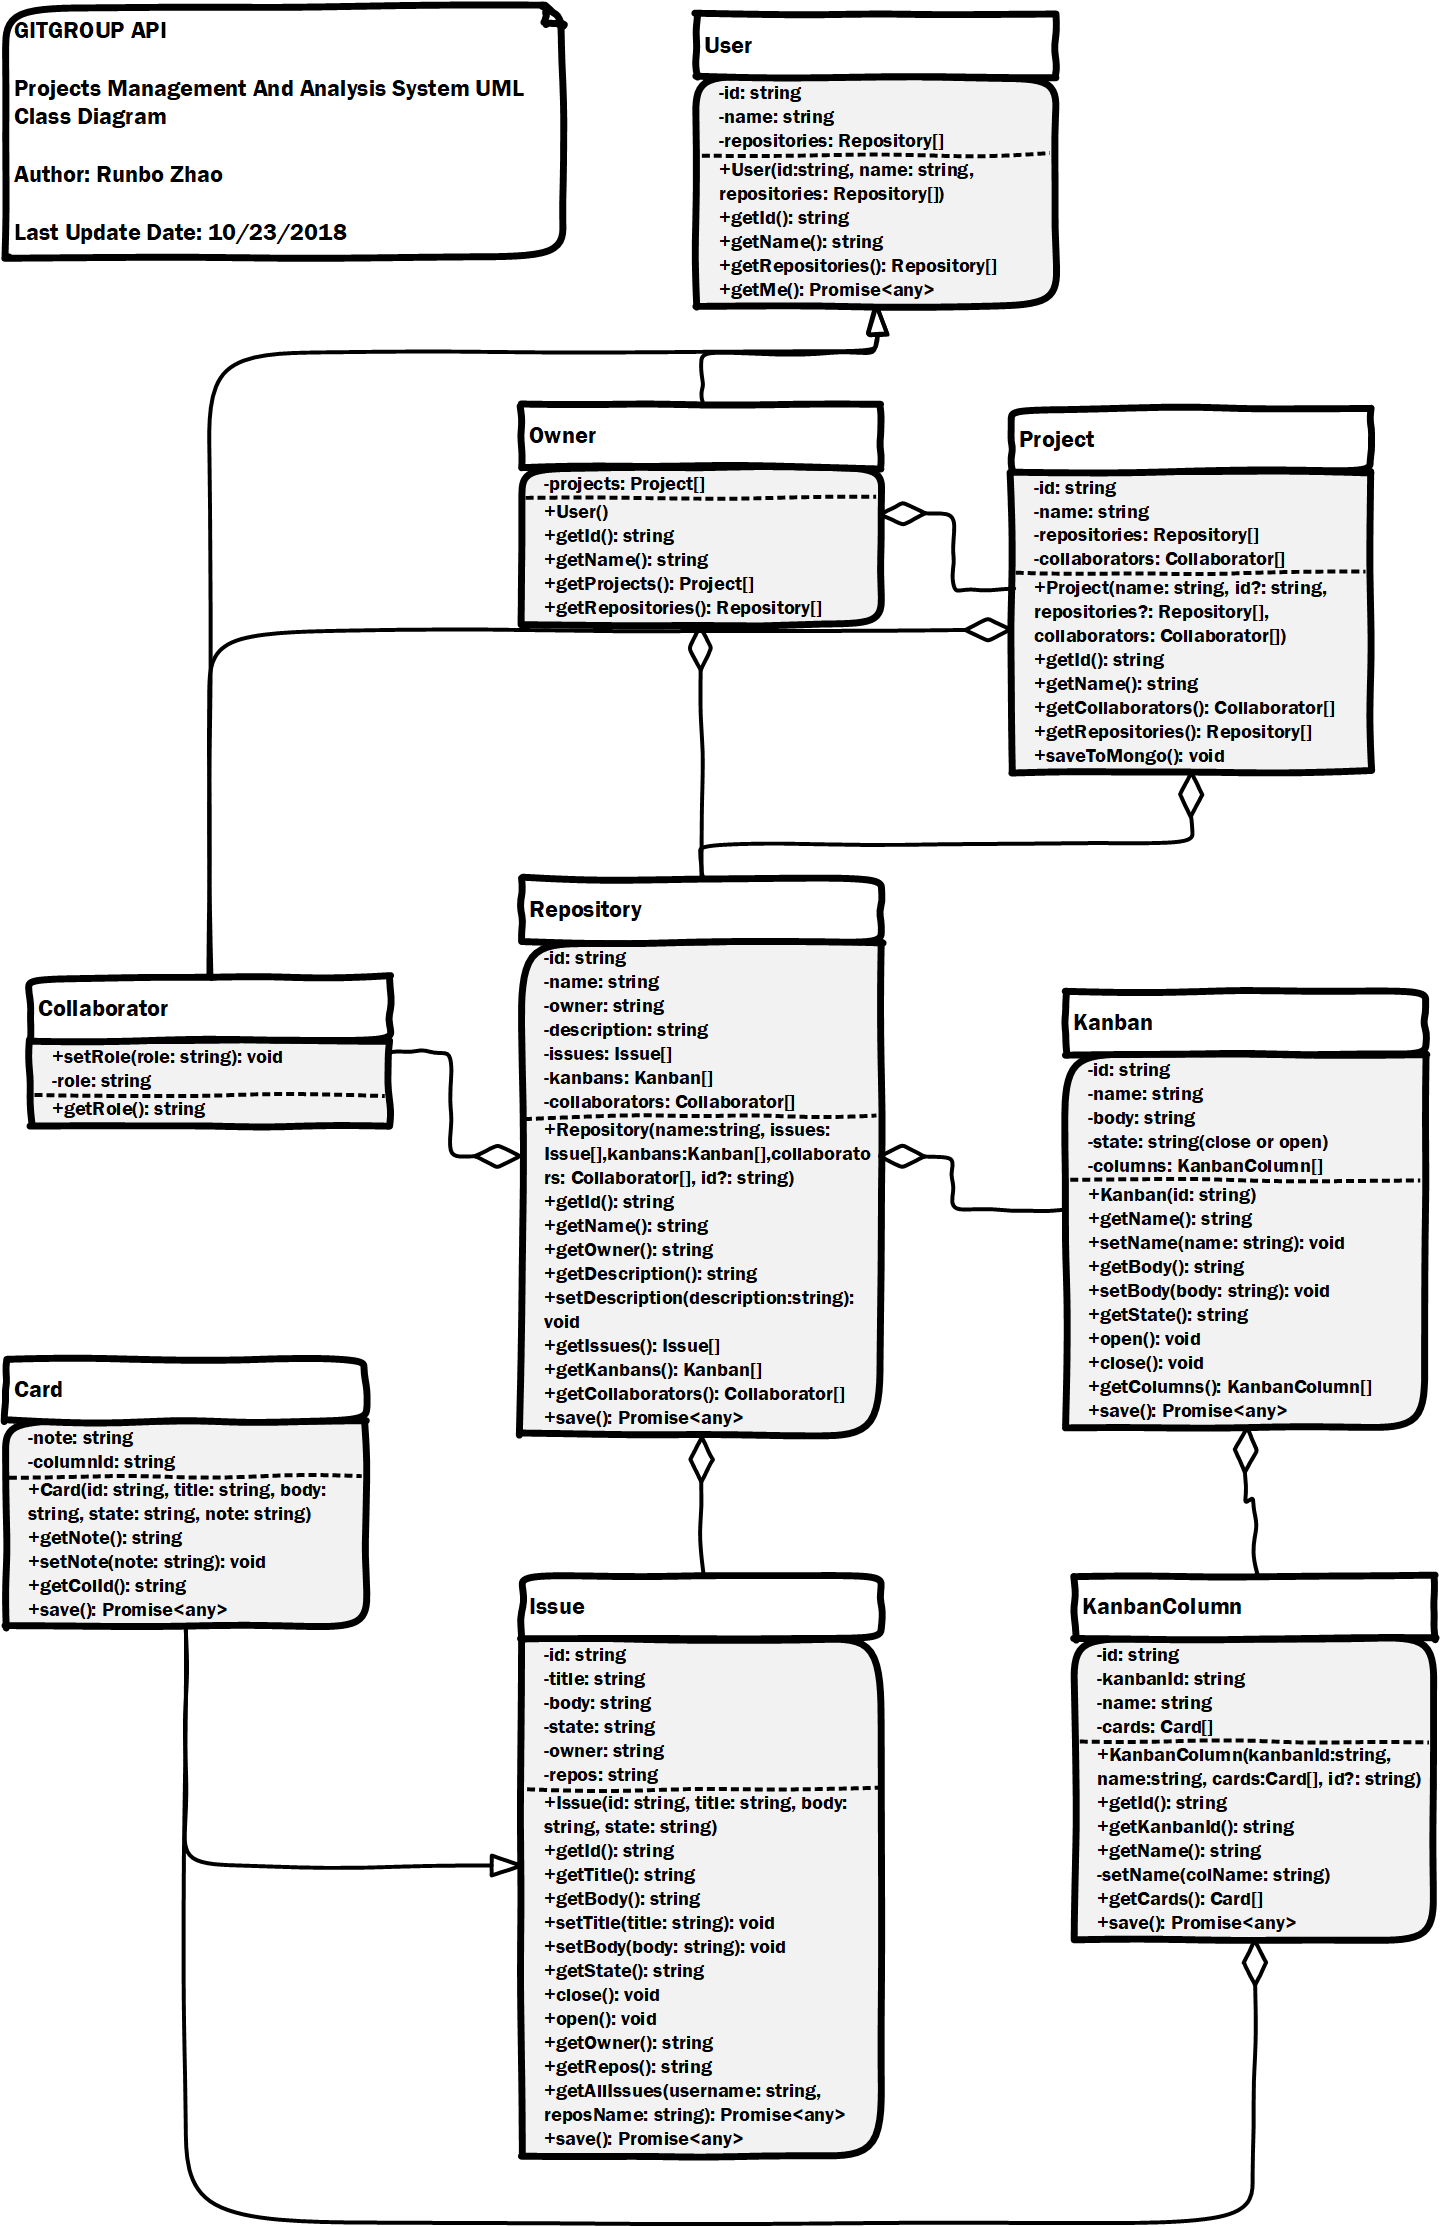
\includegraphics[width=0.6\textwidth]{./pics/ClassDiagram.png}
	\caption{UML Class Diagram (Details in Appendix A)}
\end{figure}


\chapter{System Architecture}


\cleardoublepage
\appendix
\chapter{Appendix}% <-- this title should appear on page header
\newgeometry{margin=1cm,includefoot}

\begin{figure}[h]
	\centering
	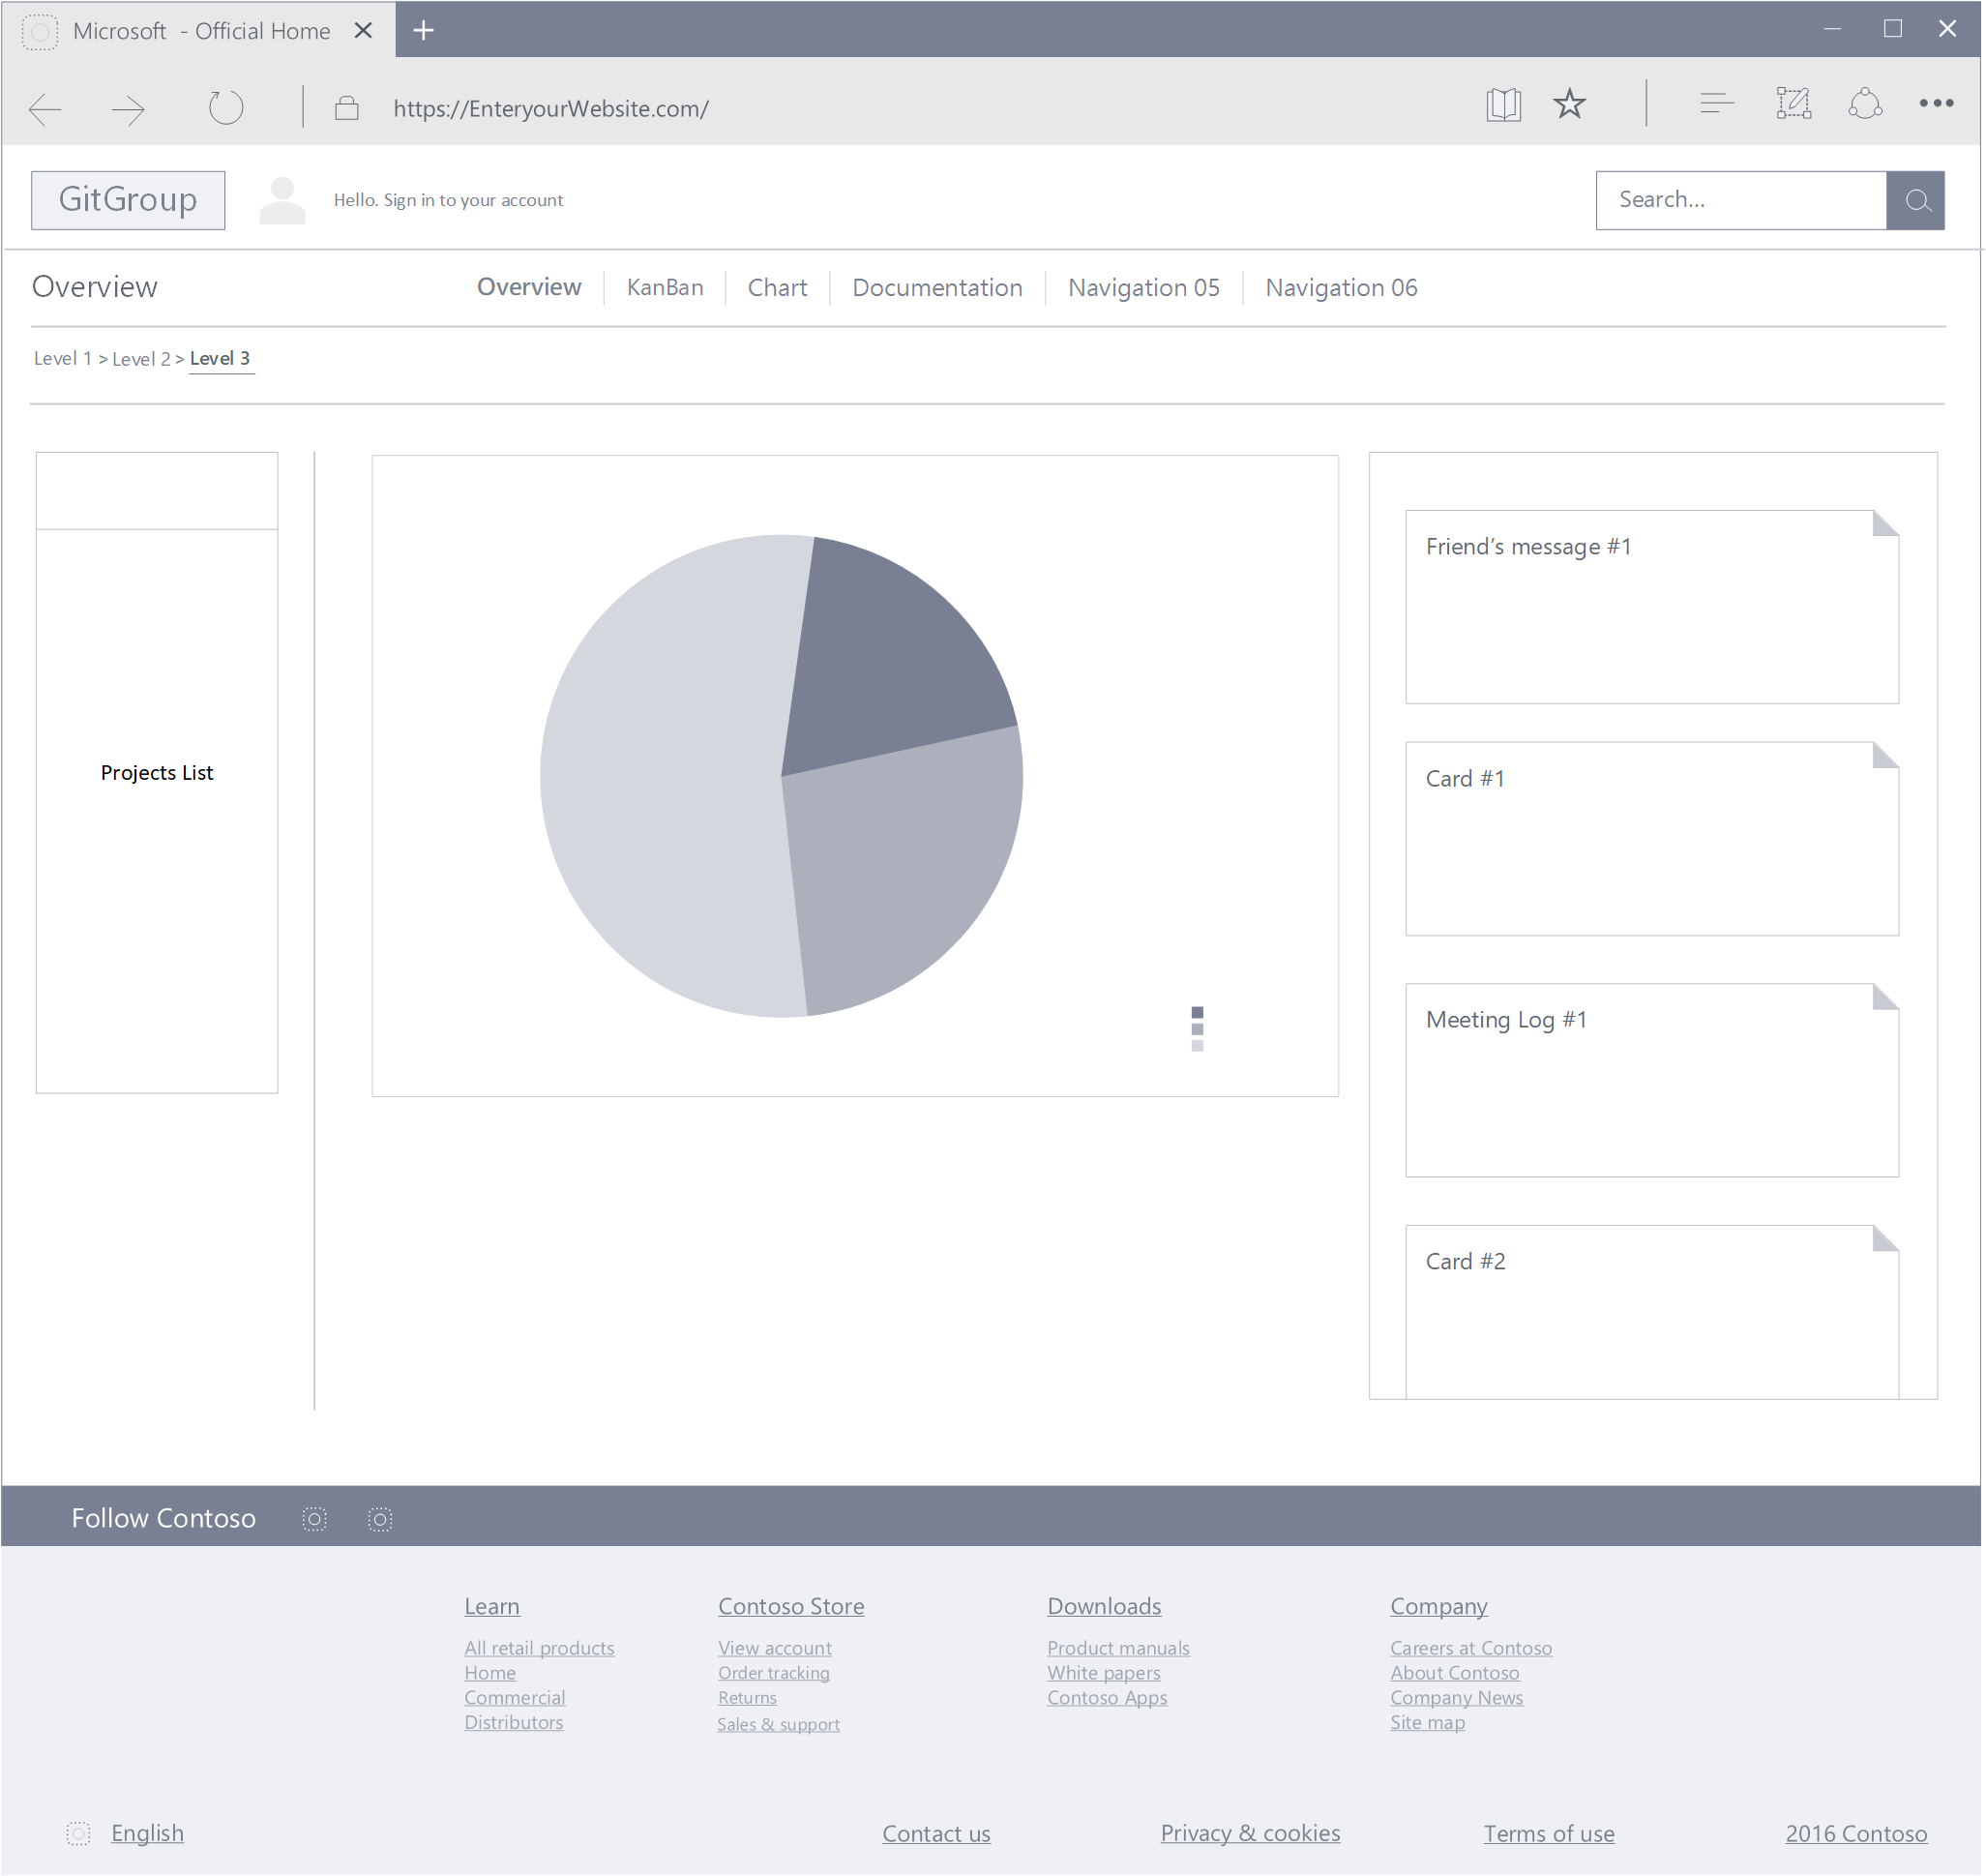
\includegraphics[width=\textwidth]{./pics/OverviewInterface.png}
	\caption{\textbf{DETAIL} Overview User Interface}
\end{figure}

\begin{figure}[h]
	\centering
	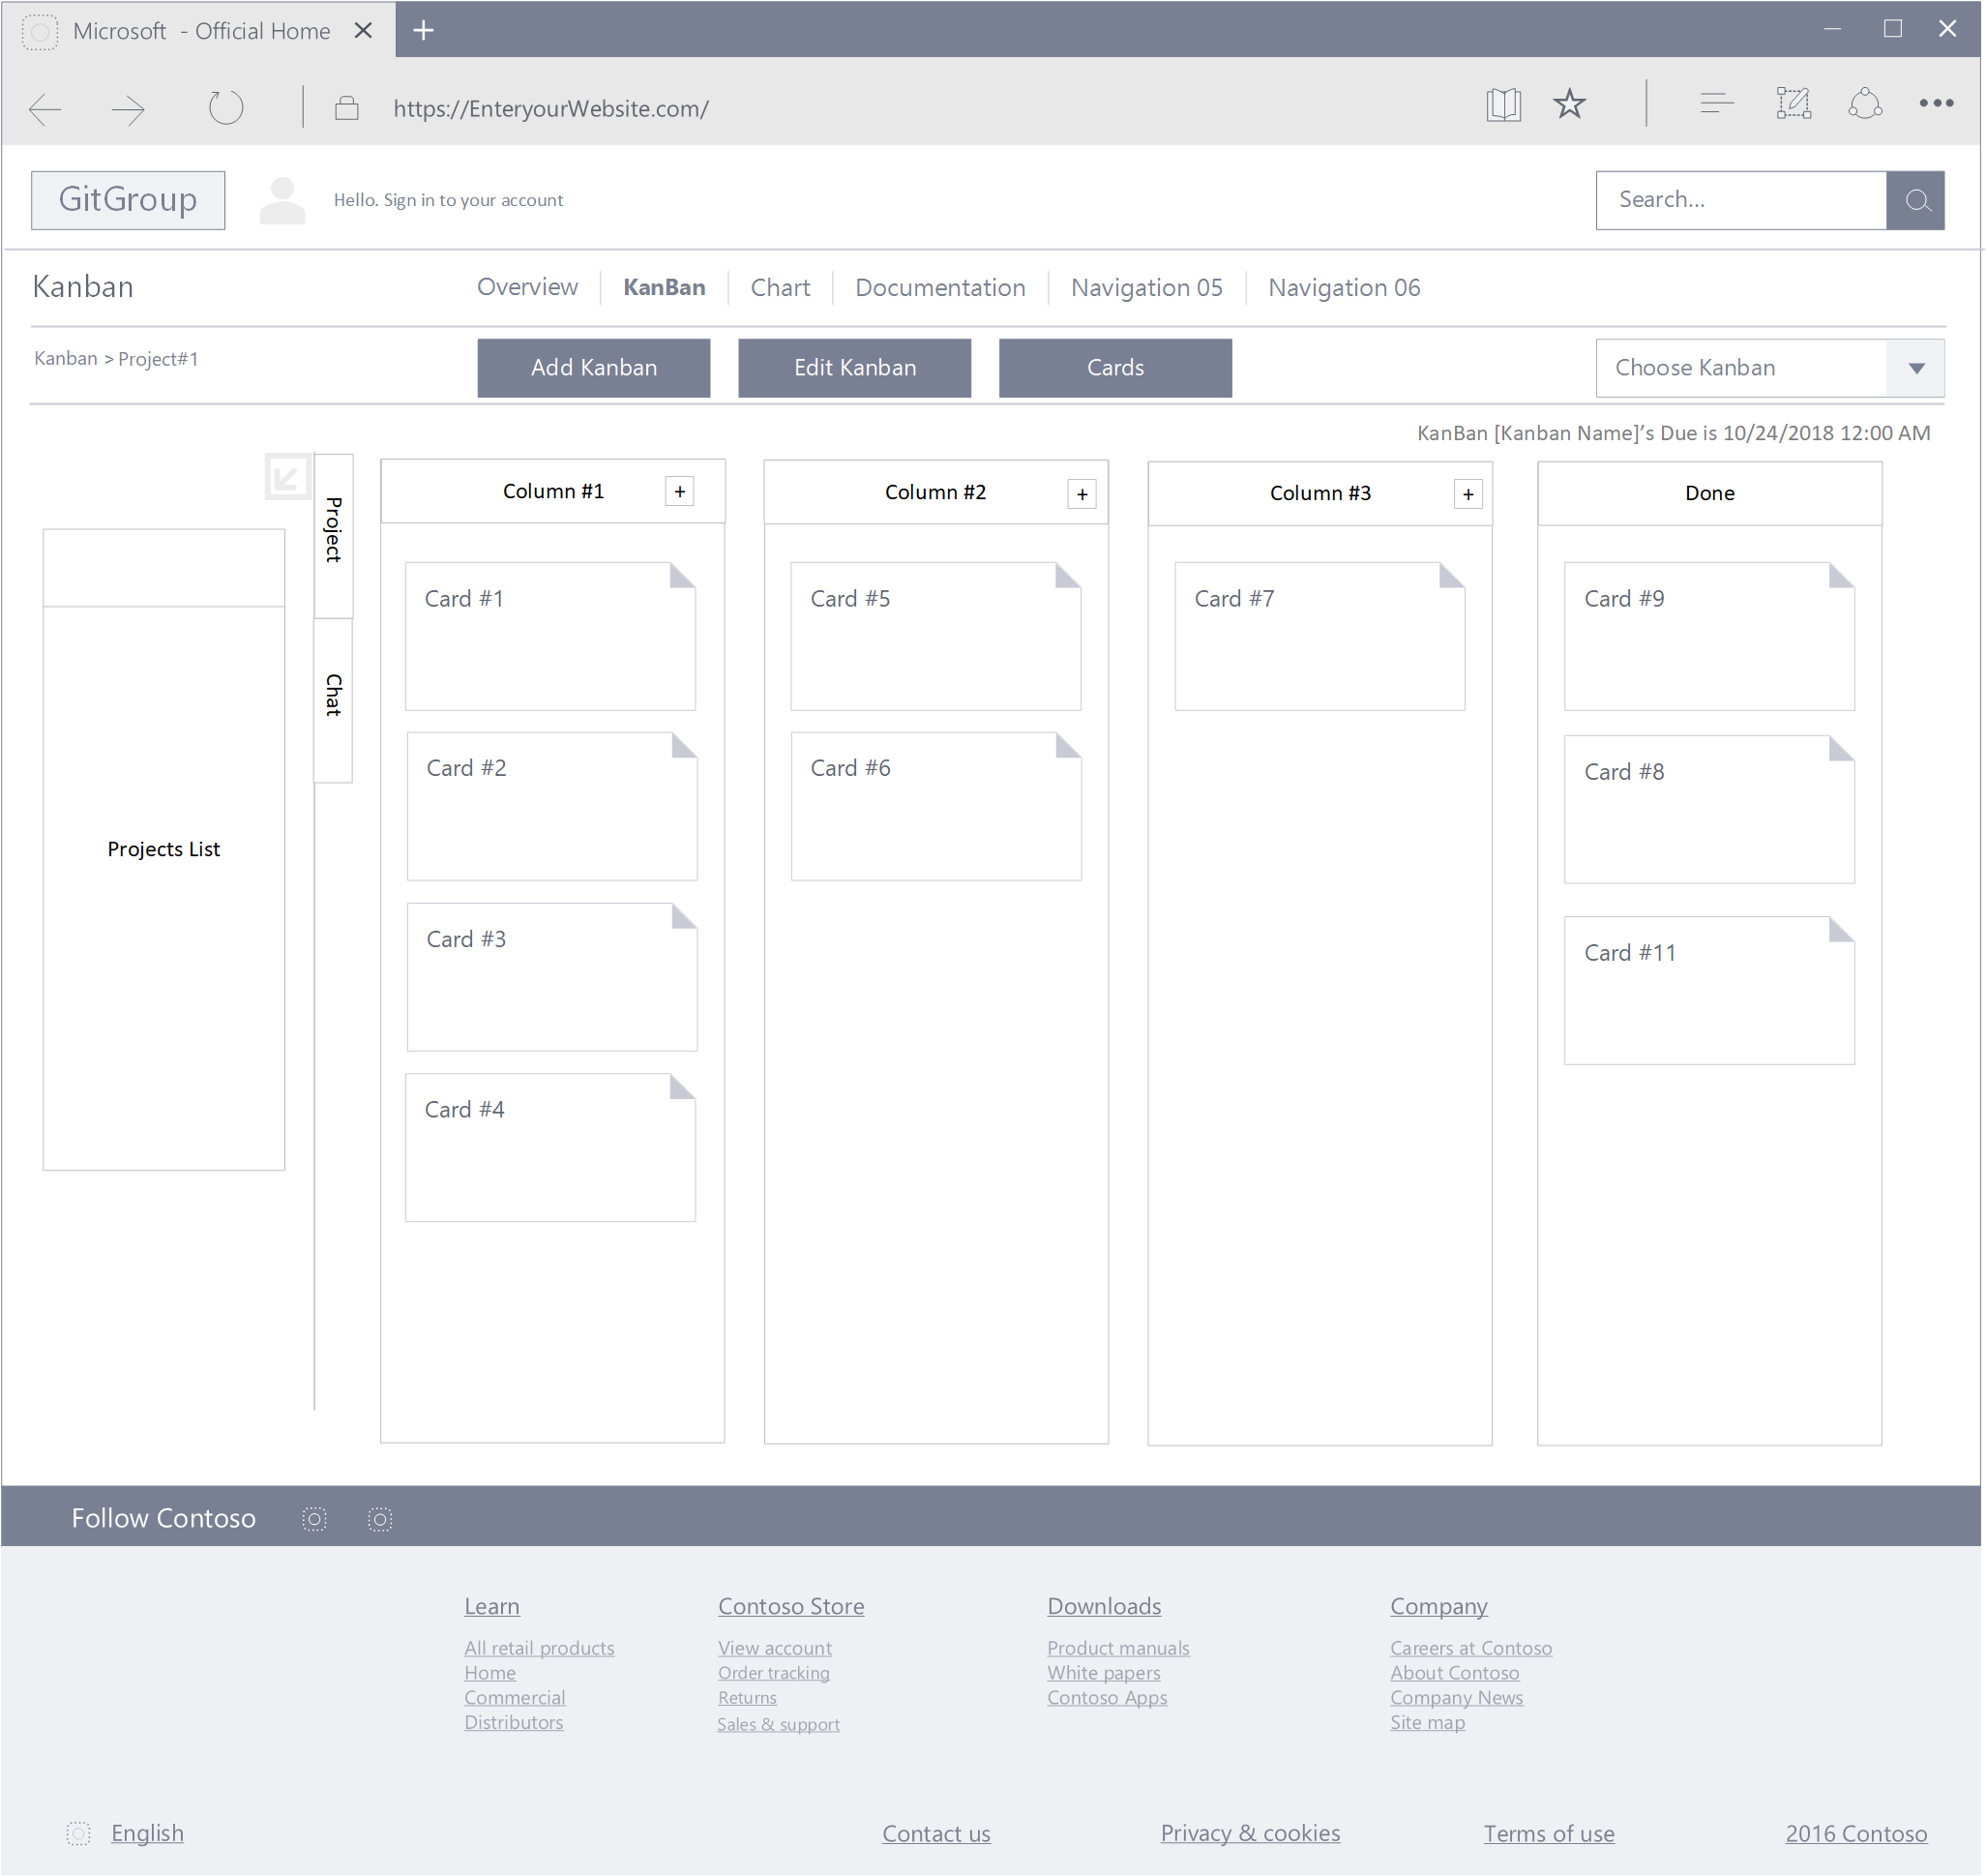
\includegraphics[width=\textwidth]{./pics/KanbanInterface.png}
	\caption{\textbf{DETAIL} KanBan User Interface}
\end{figure}

\begin{figure}[h]
	\centering
	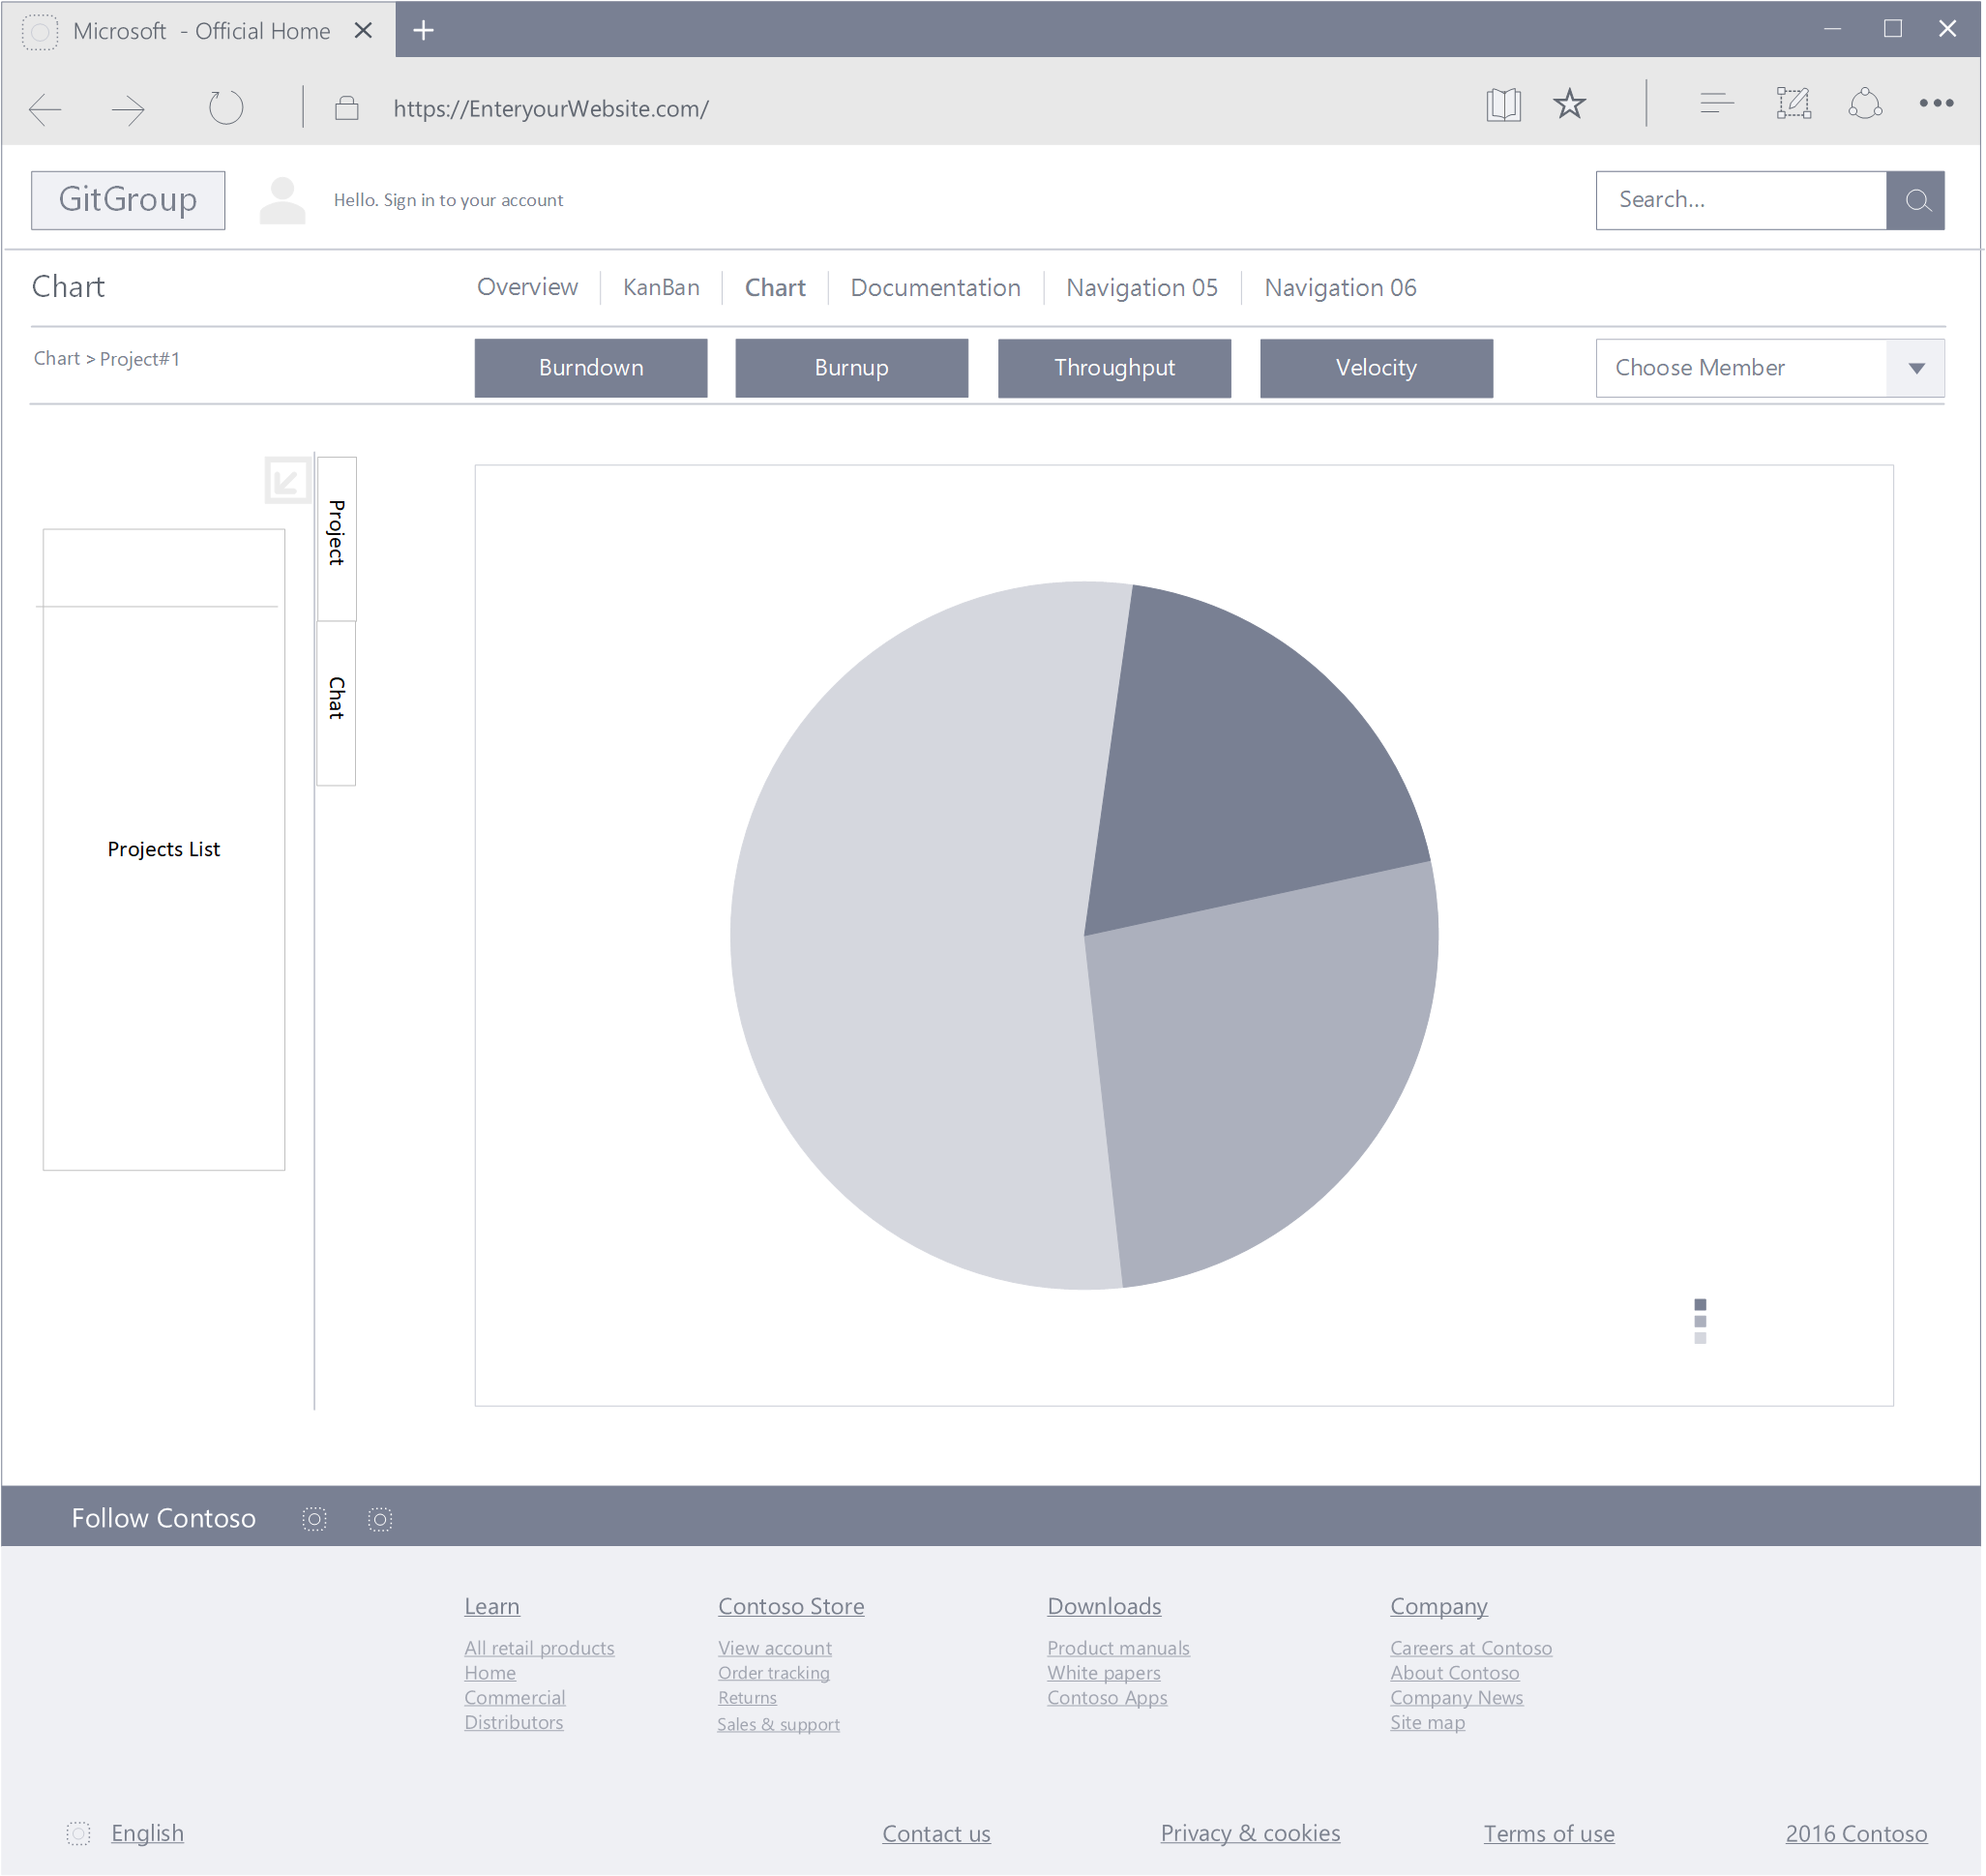
\includegraphics[width=\textwidth]{./pics/ChartInterface.png}
	\caption{\textbf{DETAIL} Chart User Interface}
\end{figure}

\begin{figure}[h]
	\centering
	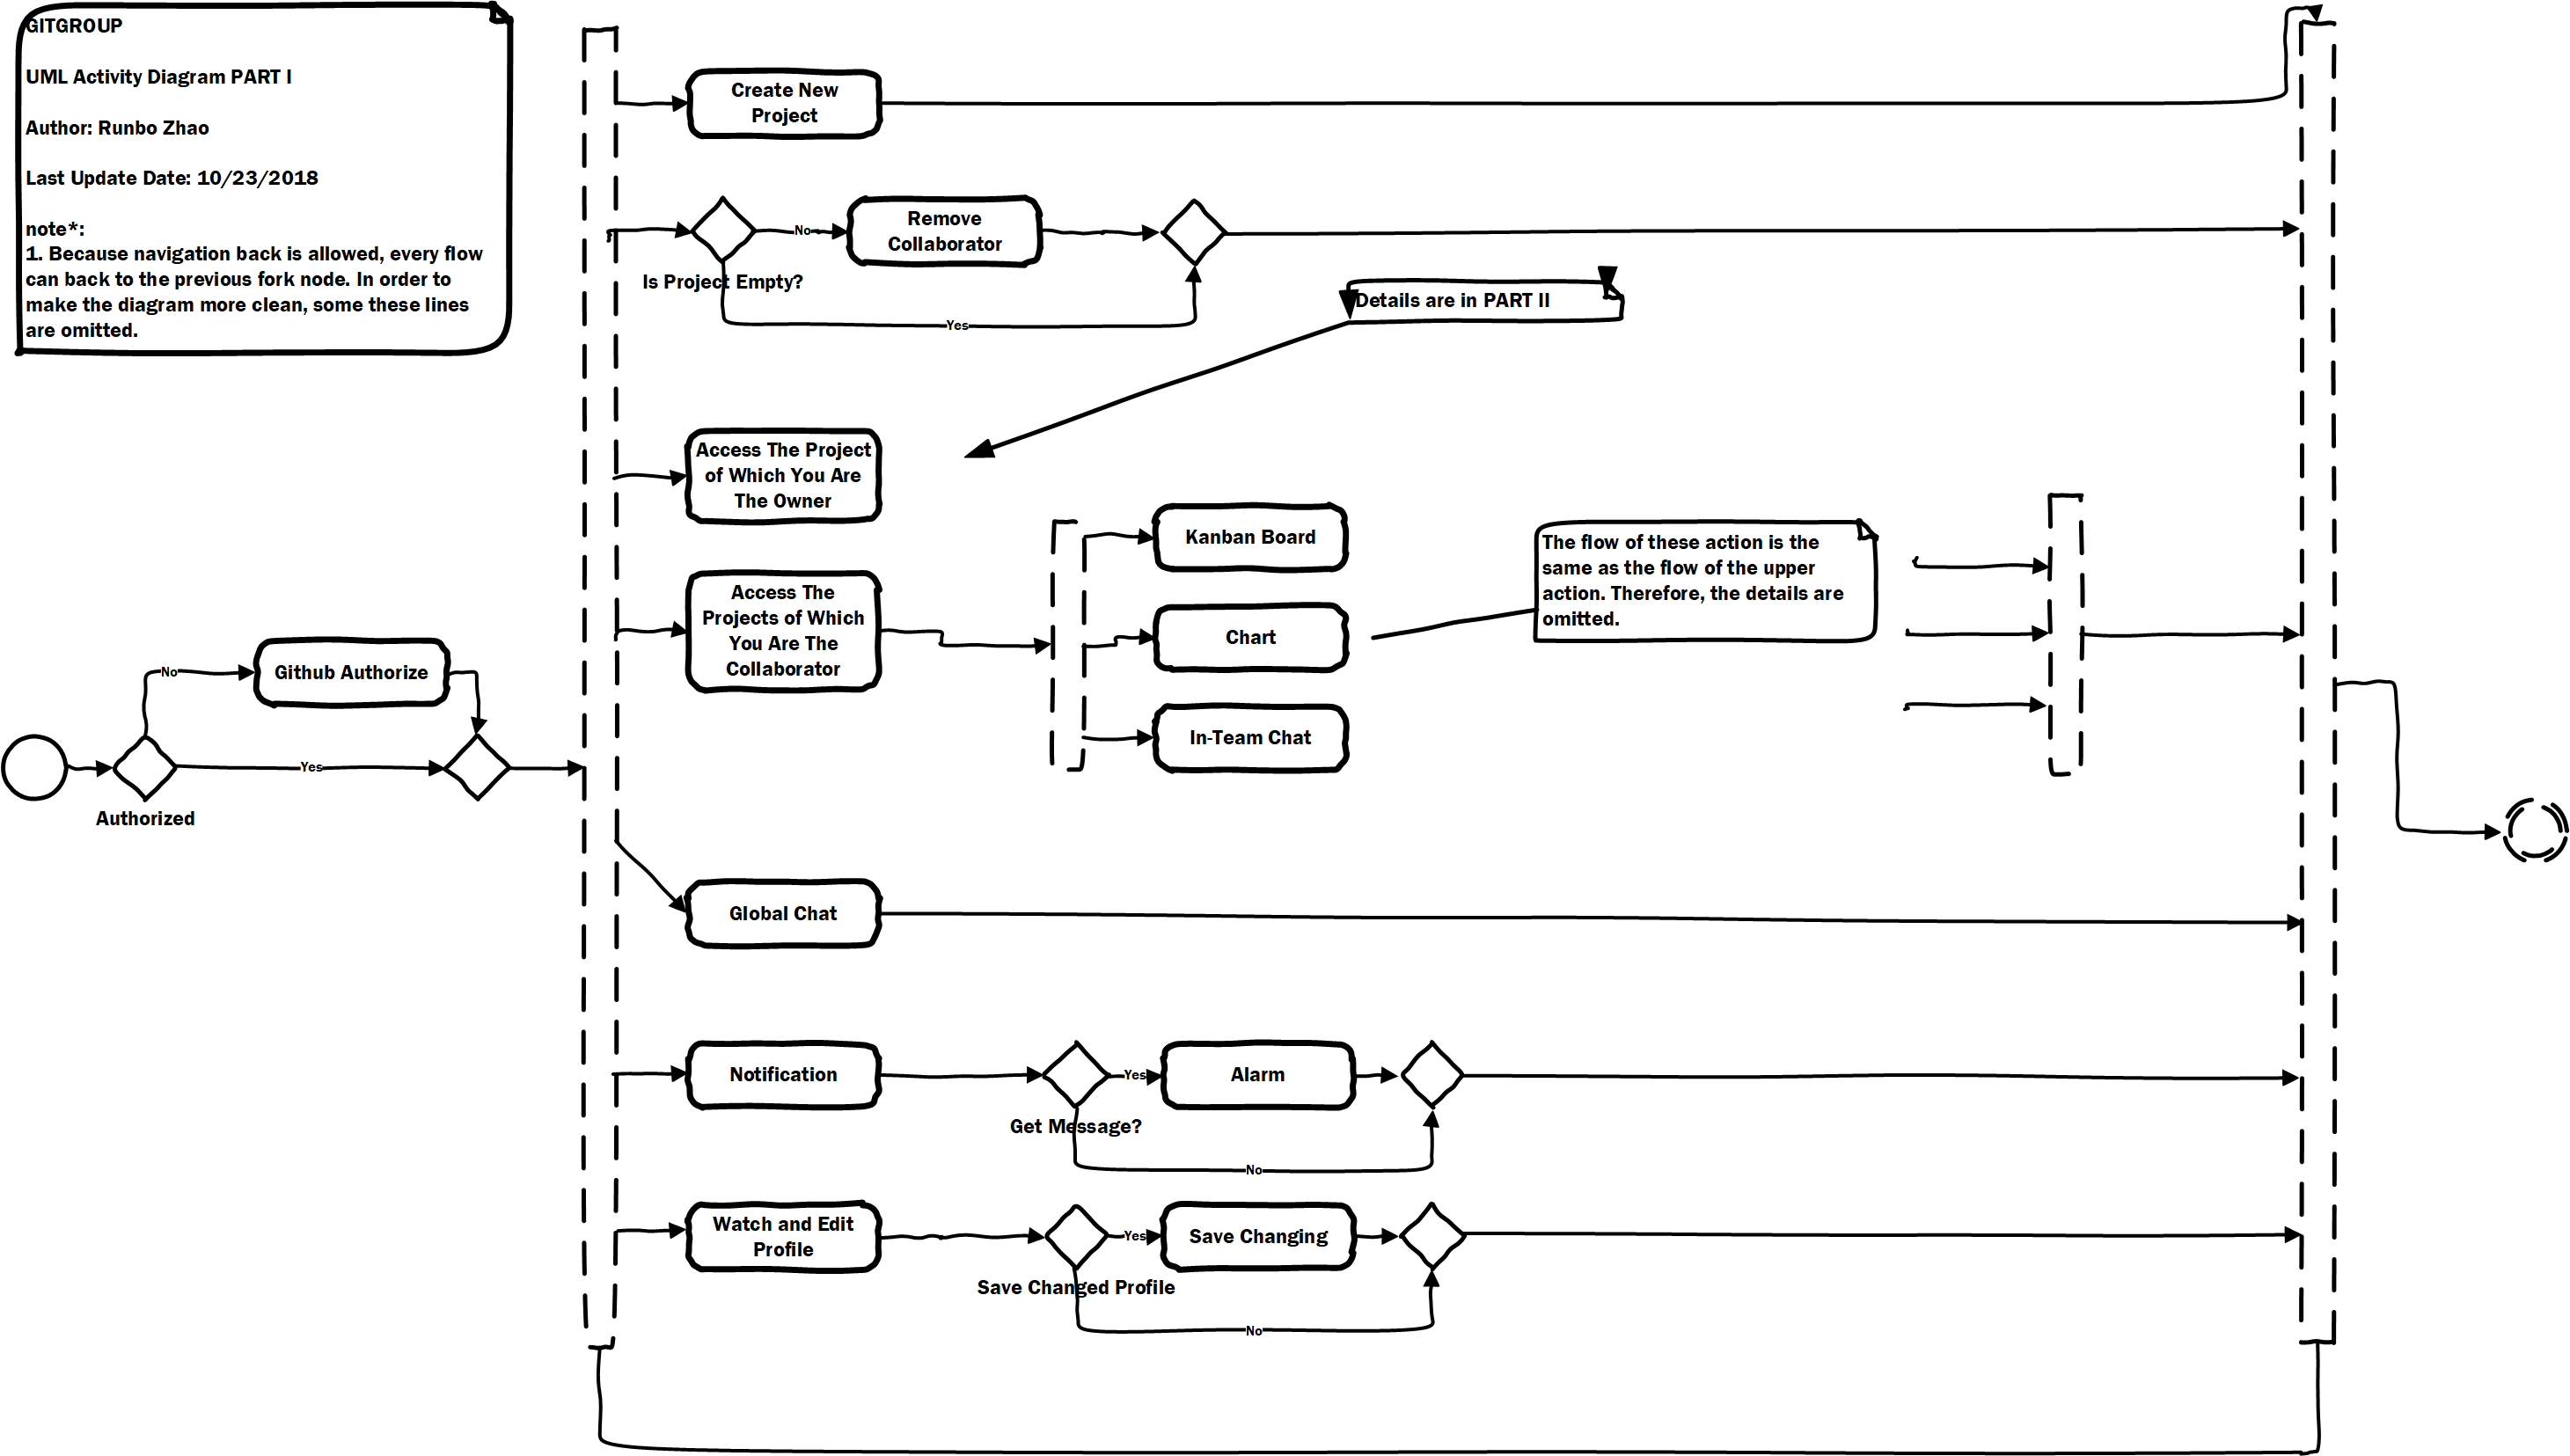
\includegraphics[scale=0.5,angle=90]{./pics/ActivatyDiagramPARTI.png}
	\caption{\textbf{DETAIL} Activity Diagram PART I}
	\label{fig1}
\end{figure}

\begin{figure}[h]
	\centering
	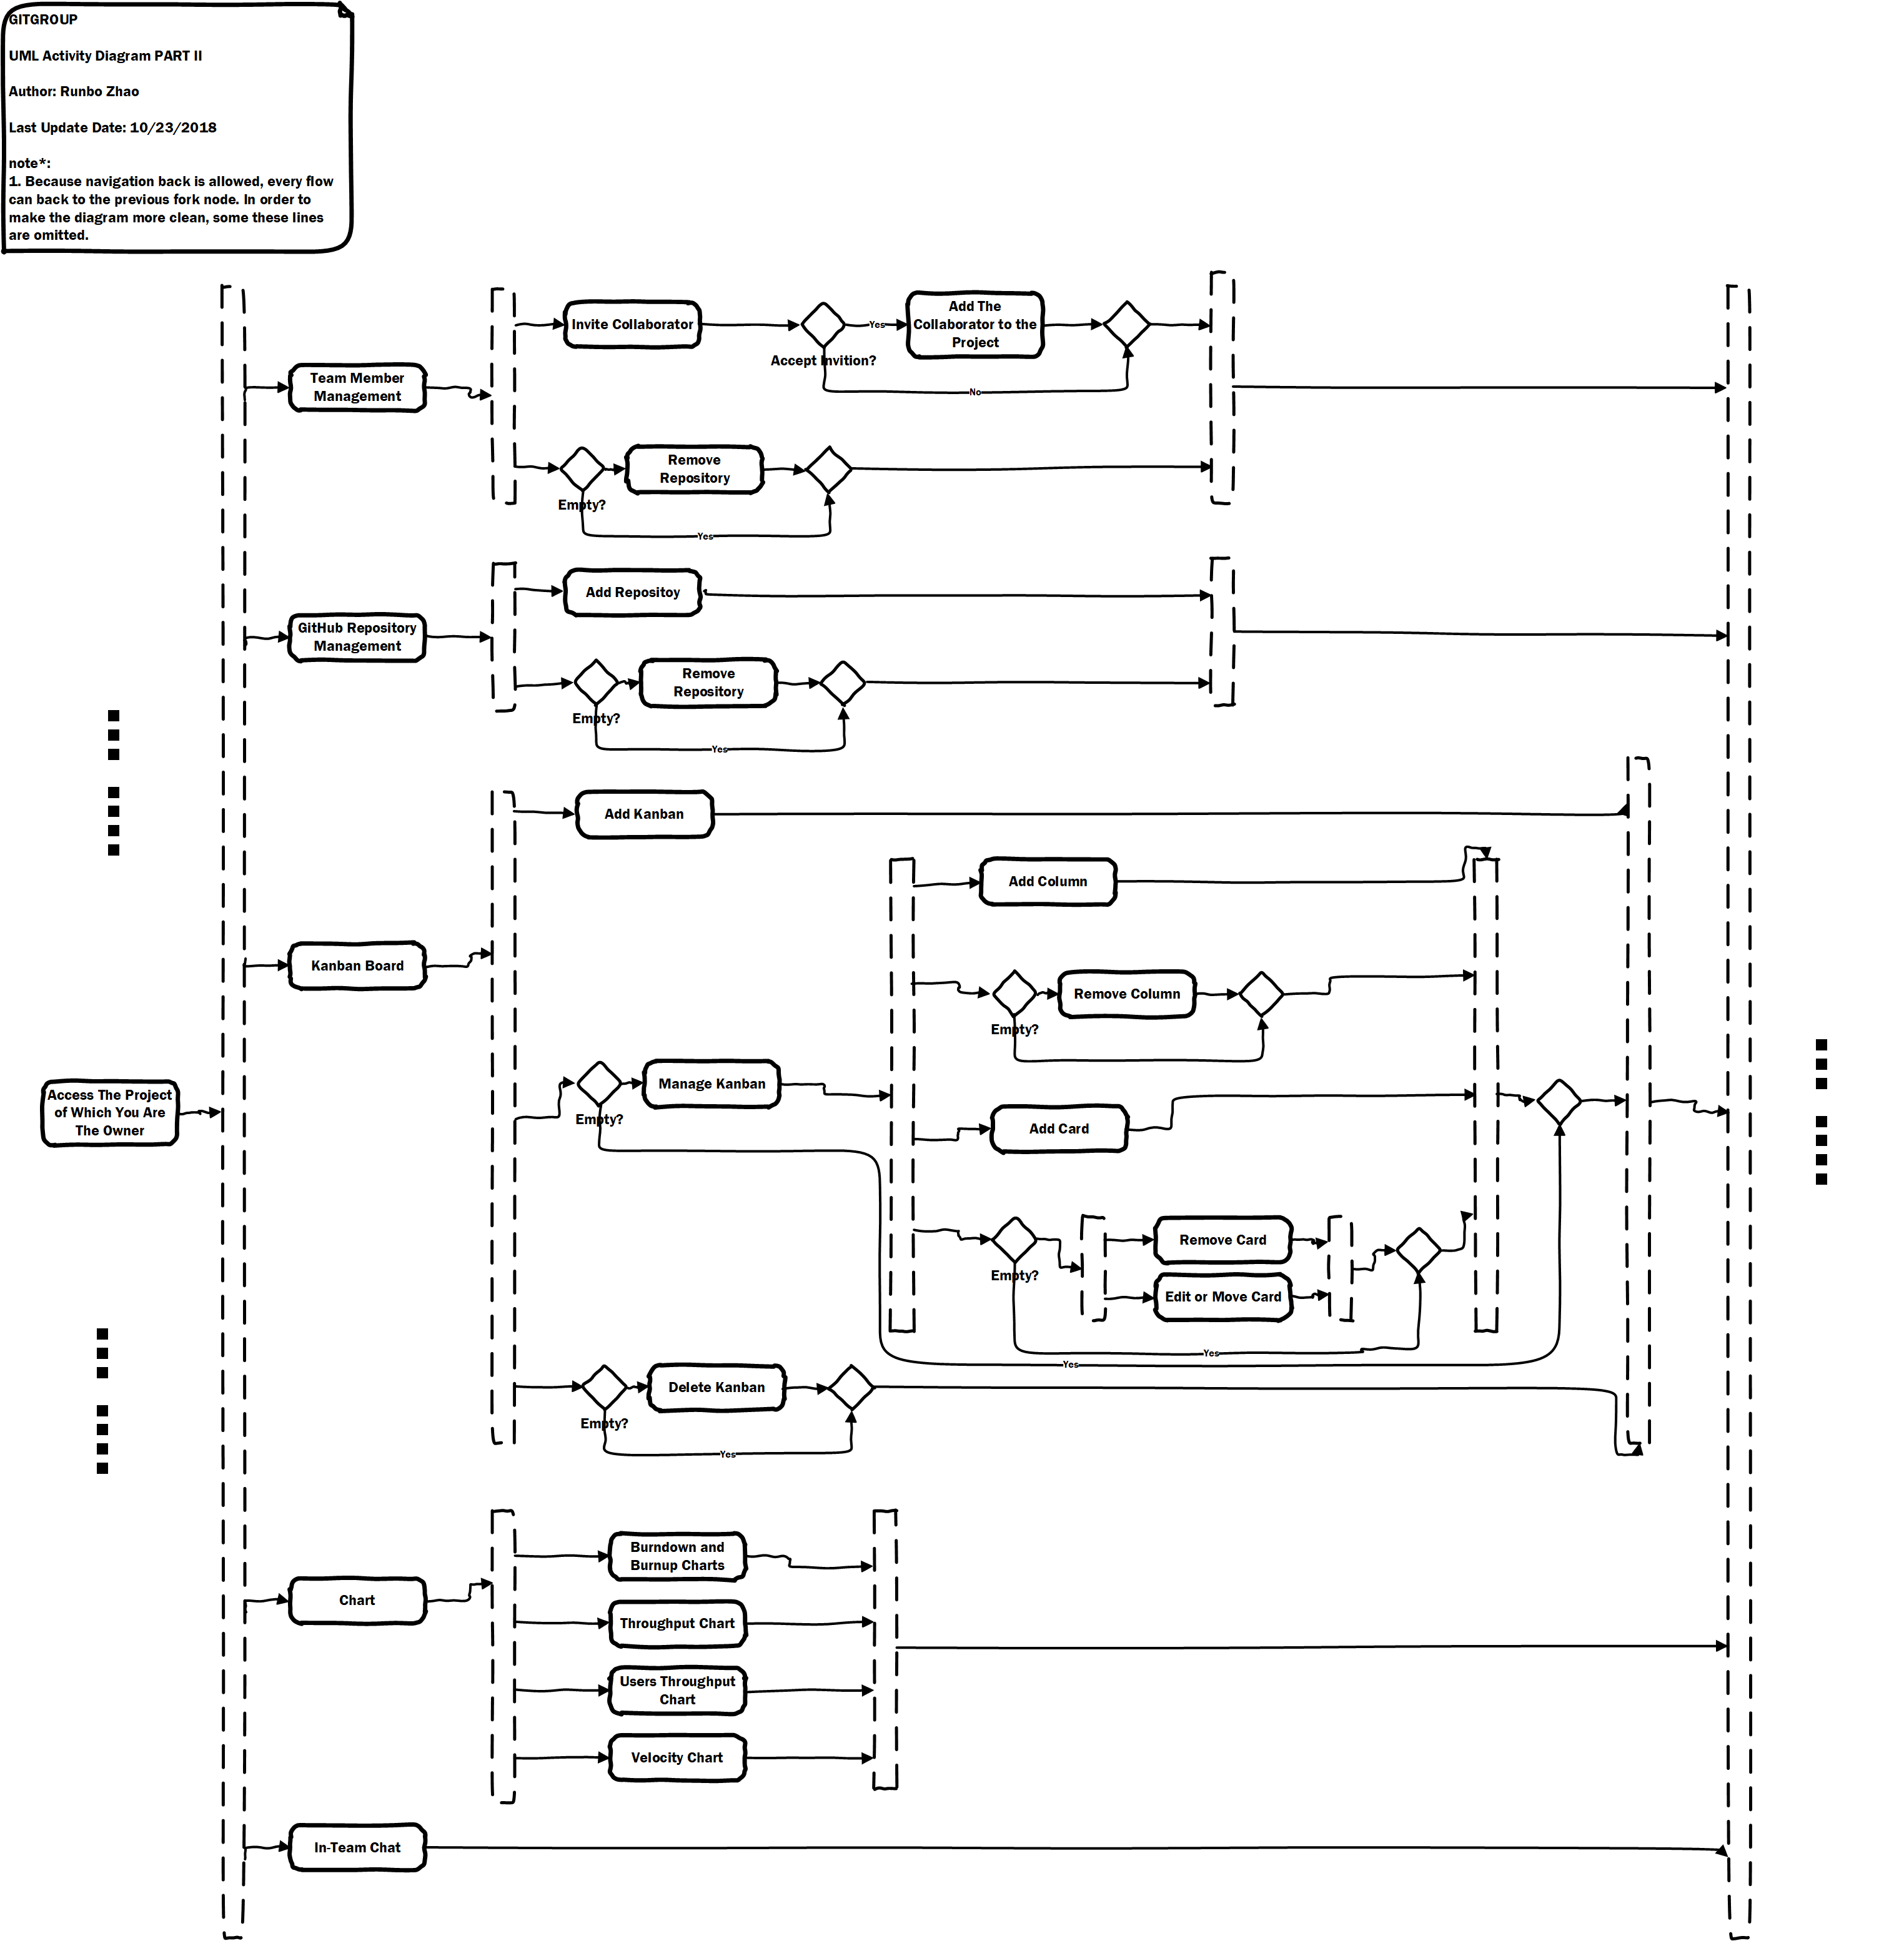
\includegraphics[width=\textwidth]{./pics/ActivatyDiagramPARTII.png}
	\caption{\textbf{DETAIL} Activity Diagram PART II}
	\label{fig2}
\end{figure}

\begin{figure}[h]
	\centering
	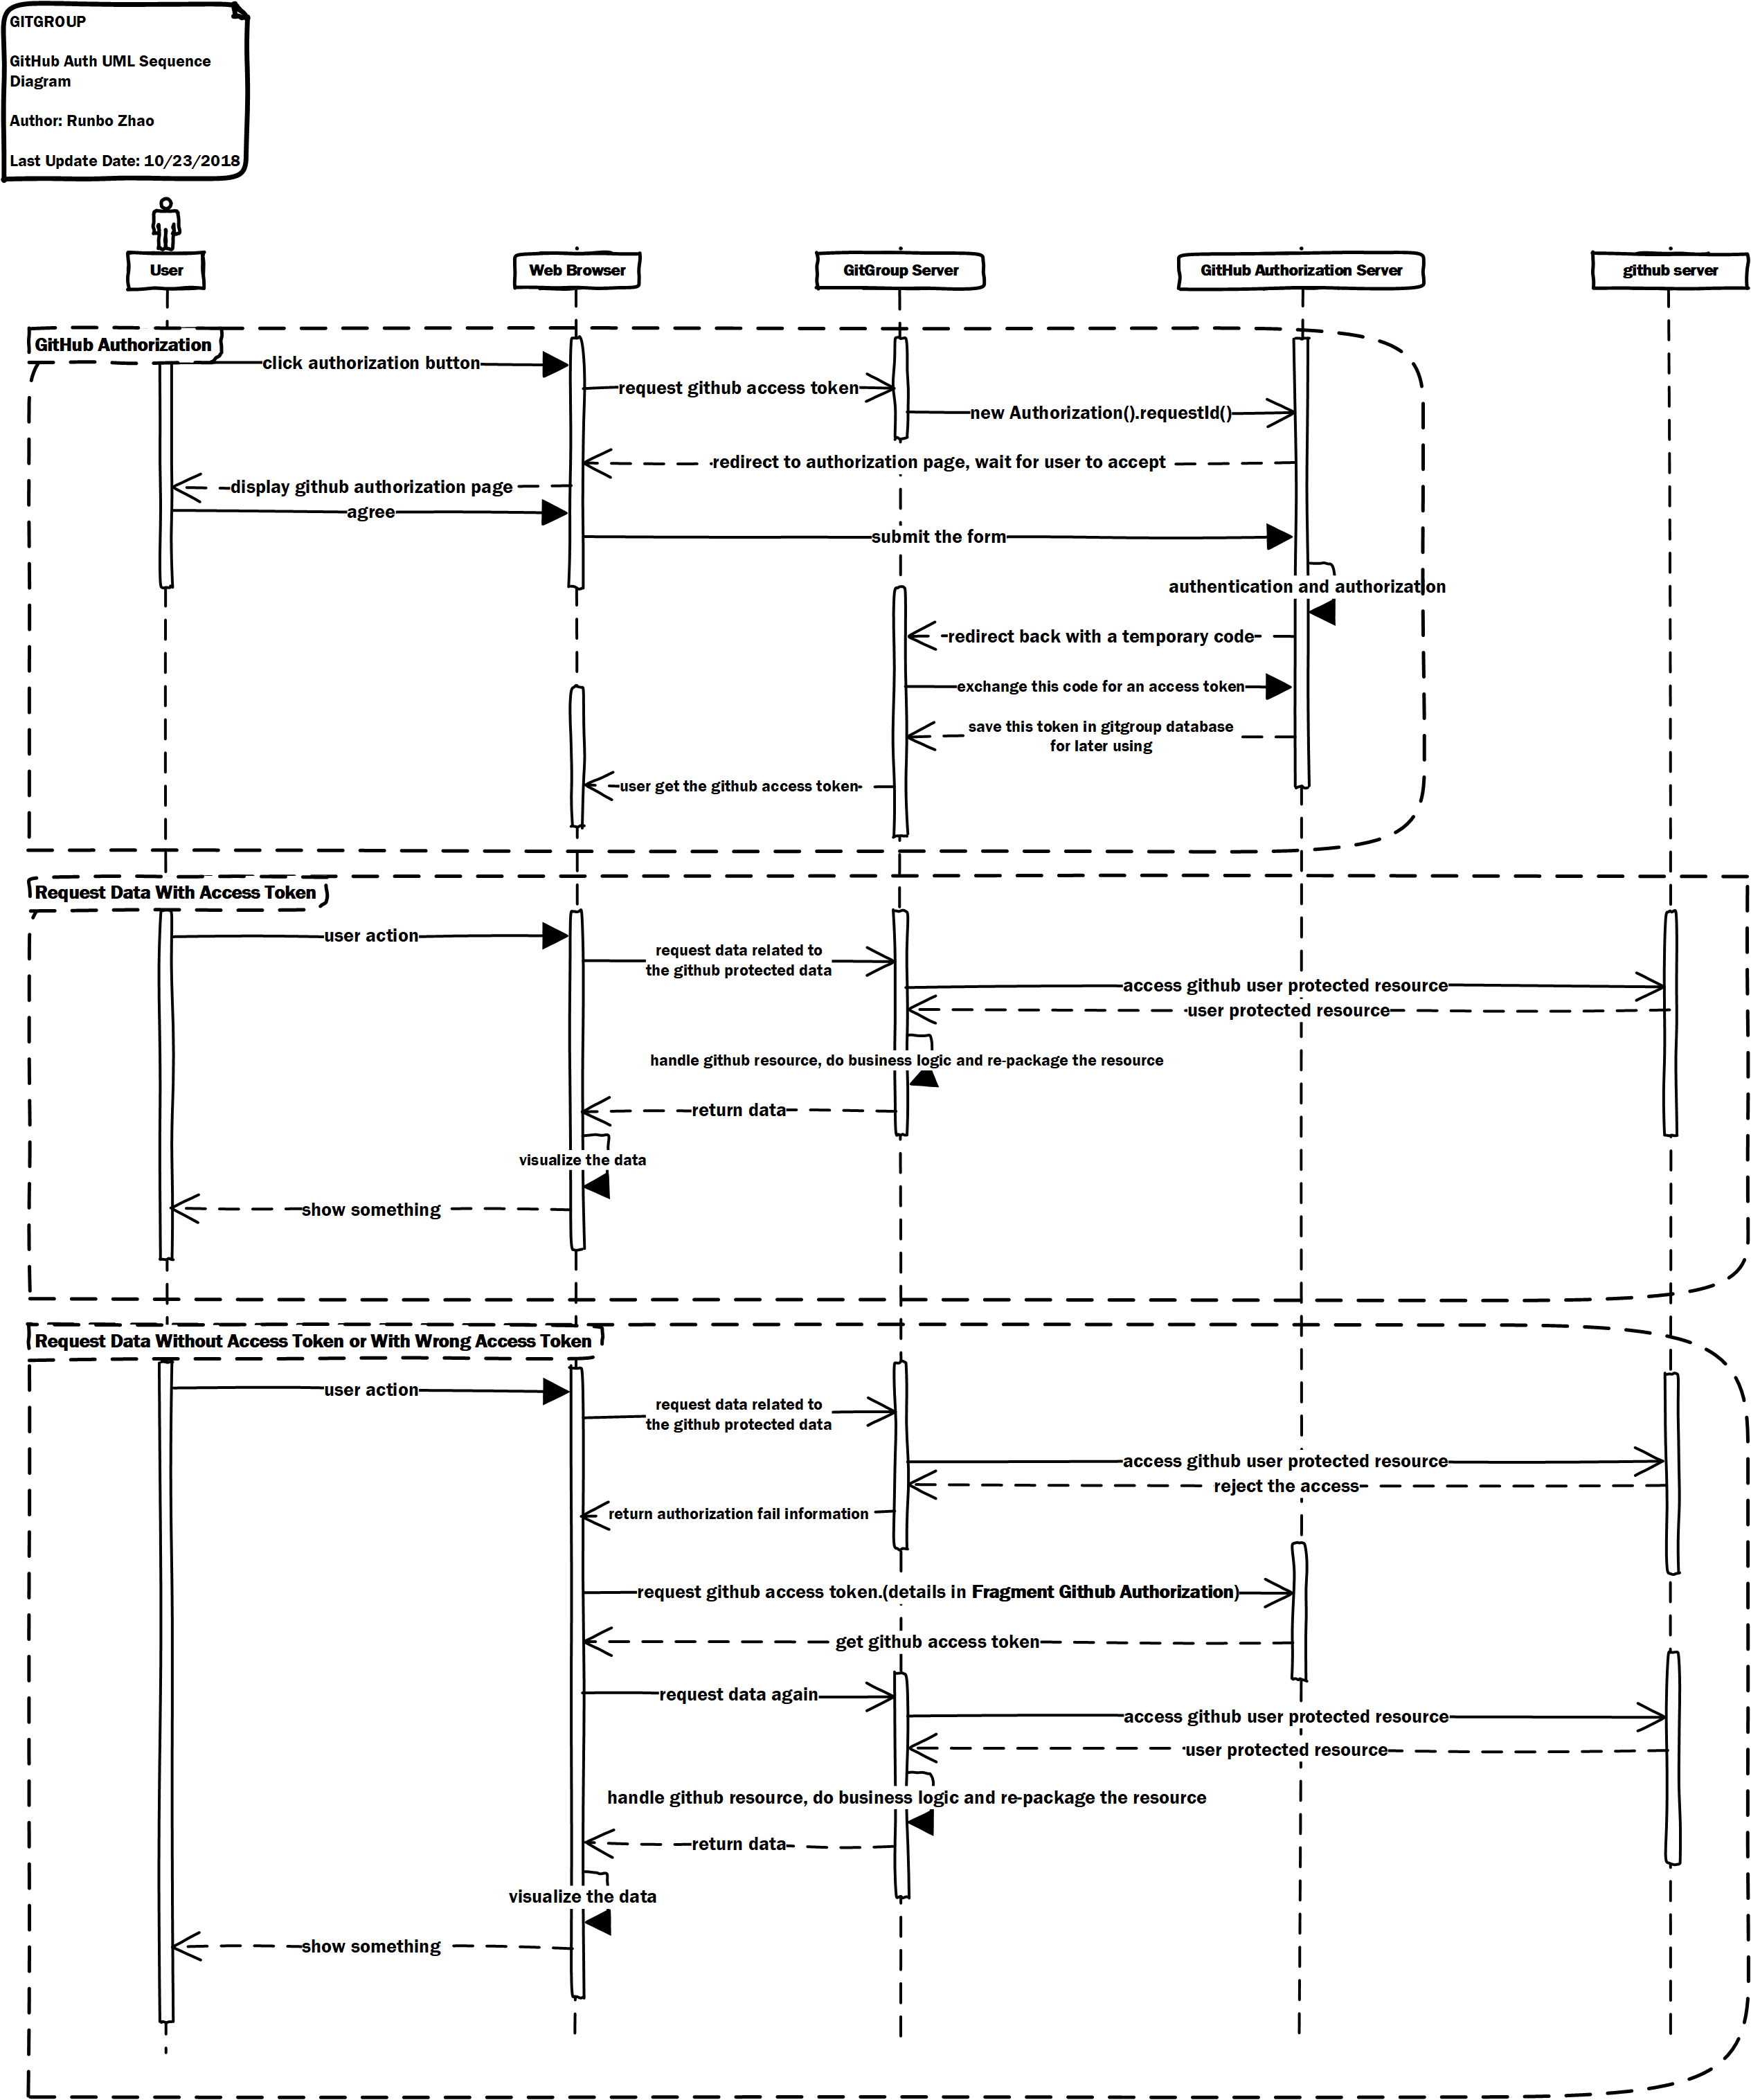
\includegraphics[width=\textwidth]{./pics/AuthSequenceDiagram.png}
	\caption{\textbf{DETAIL} Sequence Diagram For Authorization}
\end{figure}

\begin{figure}[h]
	\centering
	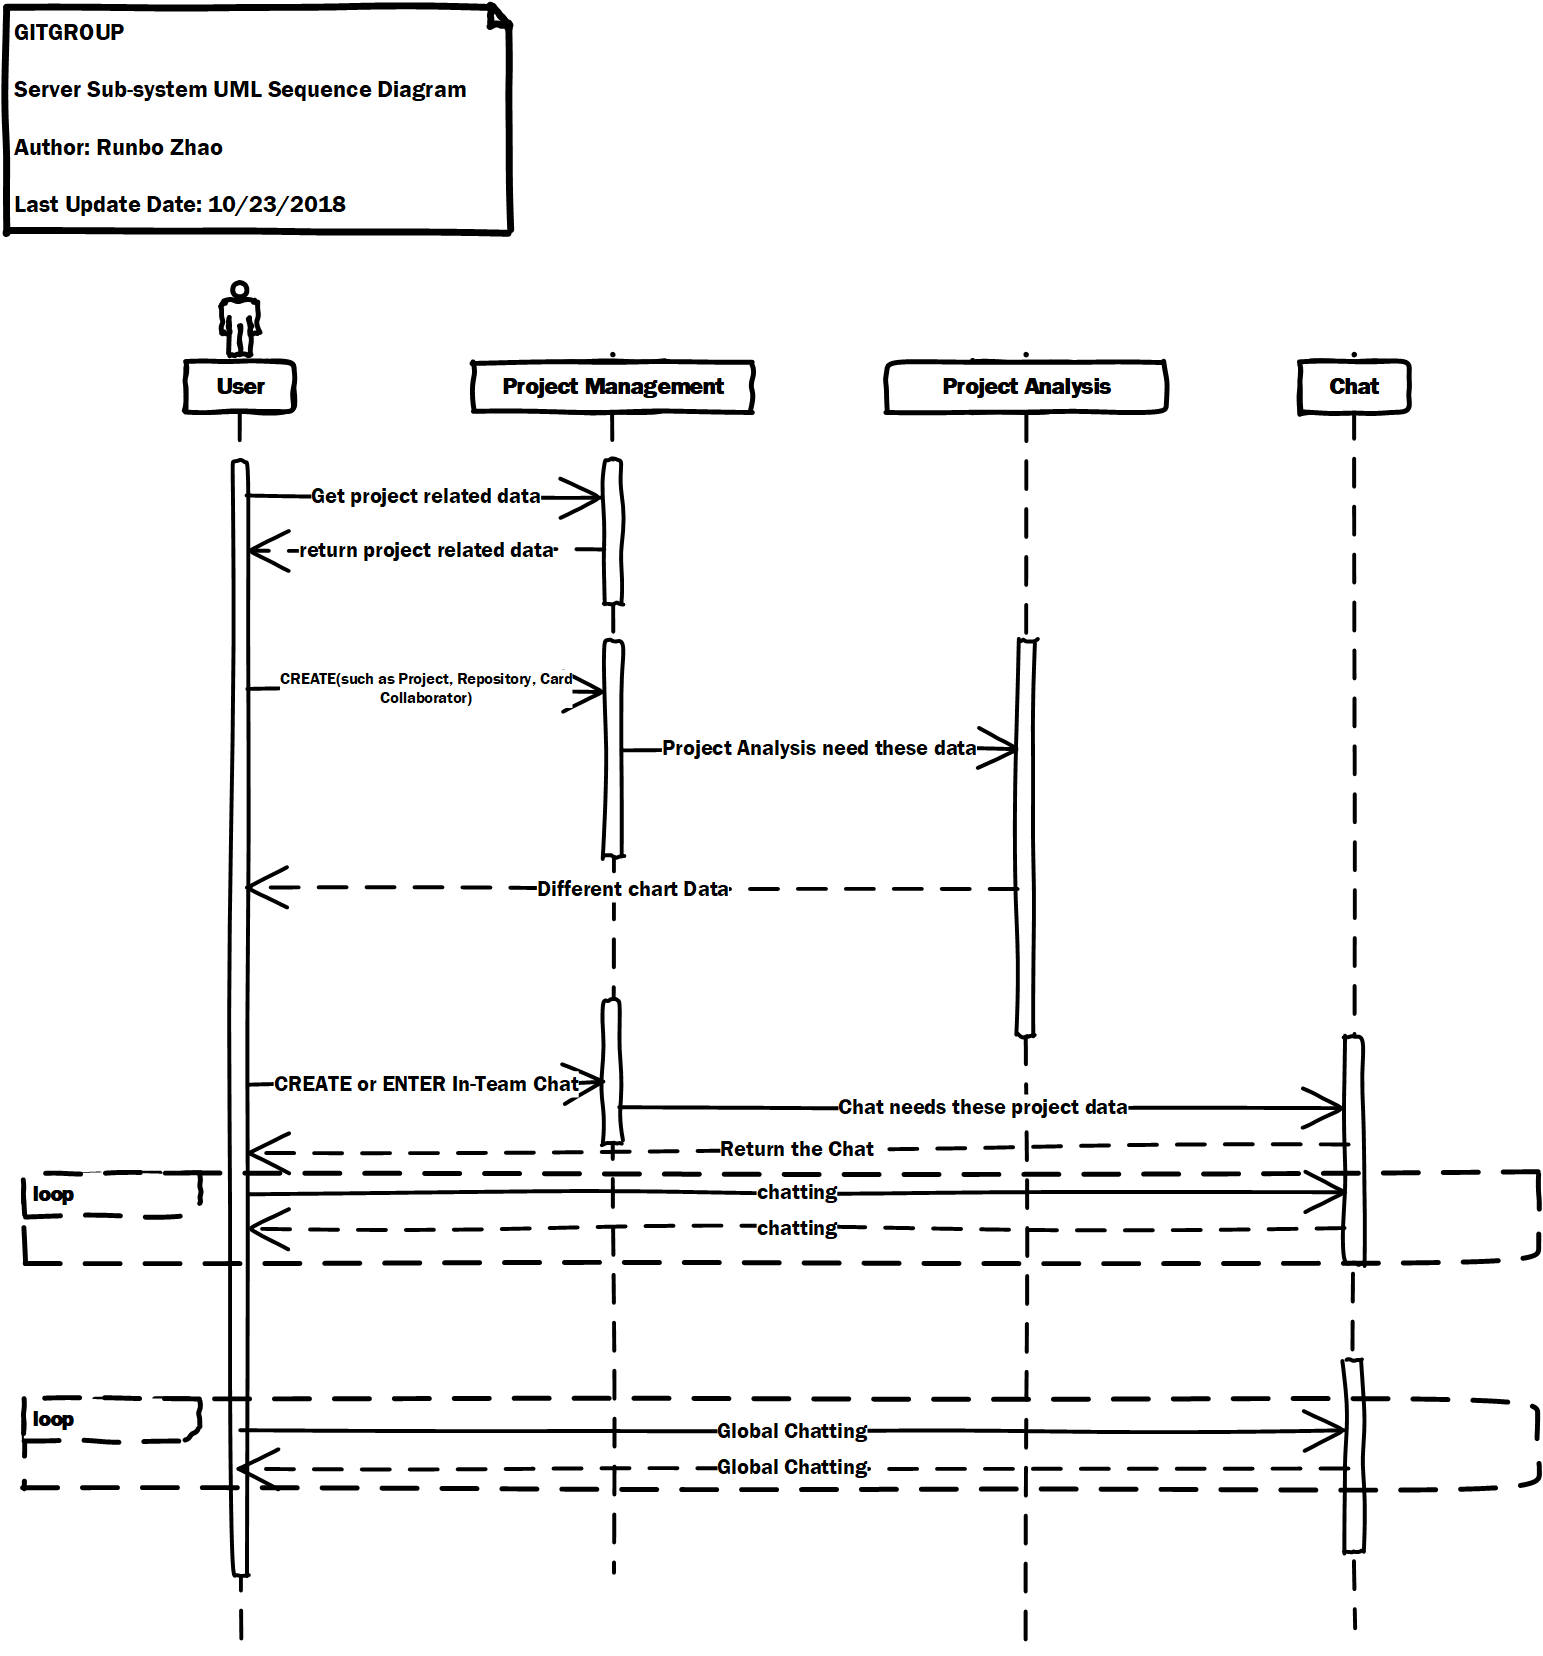
\includegraphics[width=\textwidth]{./pics/SubSysSequenceDiagram.png}
	\caption{\textbf{DETAIL} Sequence Diagram For Sub-Systems}
\end{figure}

\begin{figure}[h]
	\centering
	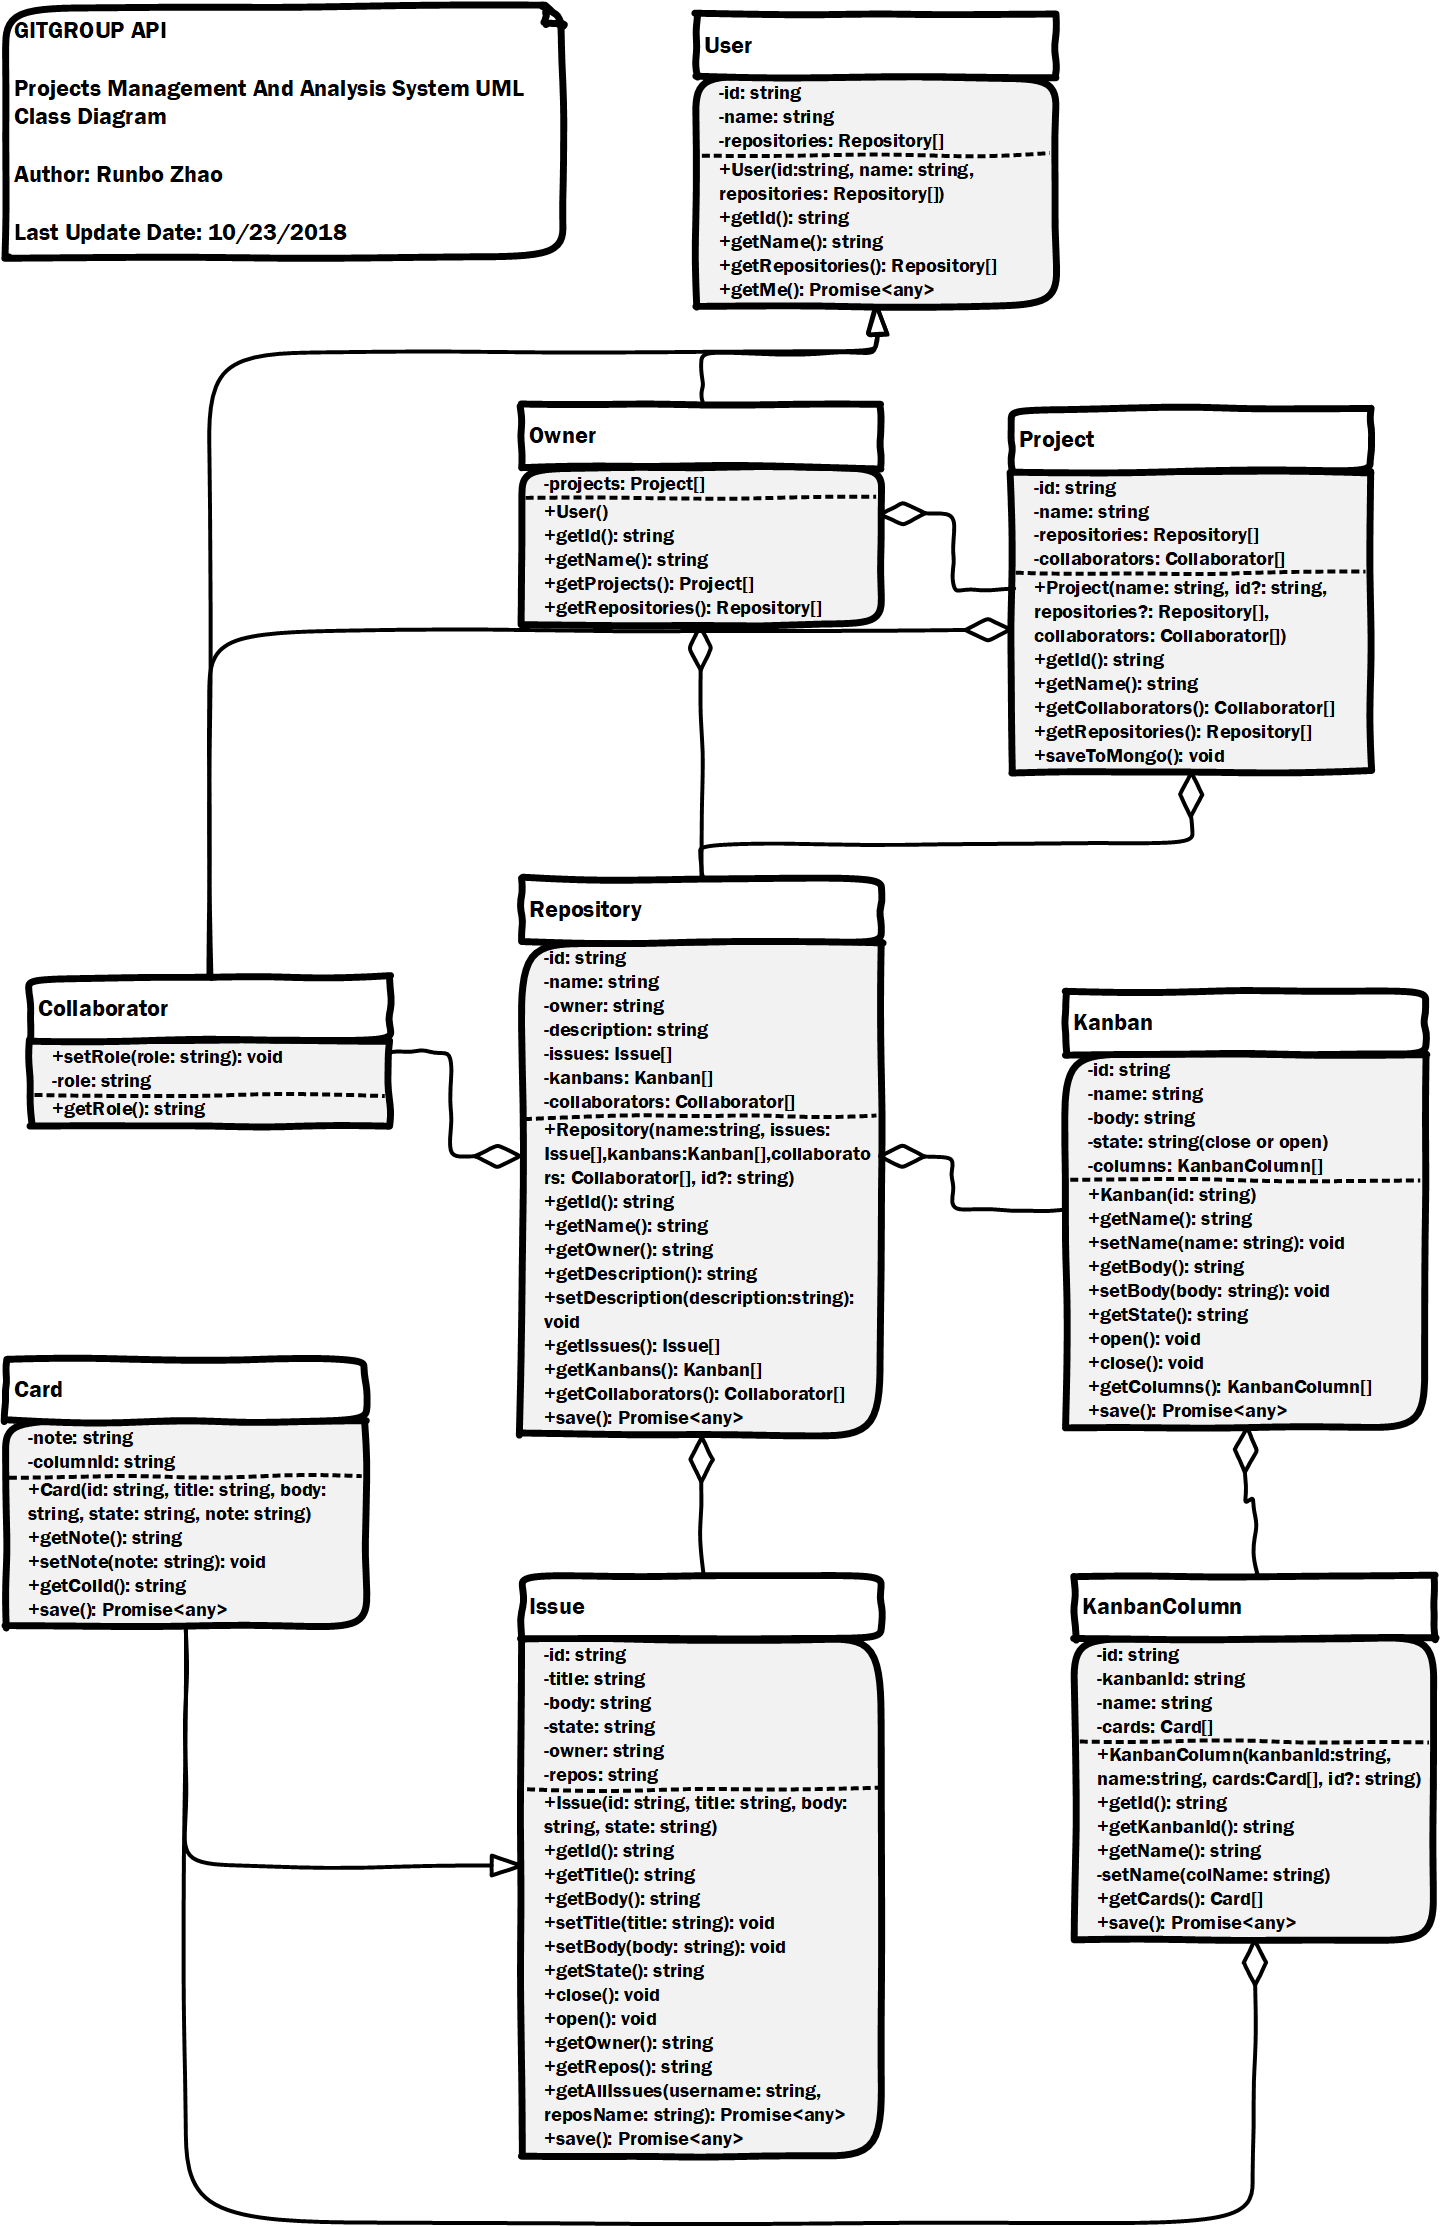
\includegraphics[height=0.95\textheight]{./pics/ClassDiagram.png}
	\caption{\textbf{DETAIL} UML Class Diagram}
\end{figure}


\cleardoublepage
\listoffigures
\cleardoublepage
\listoftables

\begin{enumerate}
\renewcommand{\labelenumi}{{\textbf{\arabic{enumi}.}}}
\item o
\item two
\item three
\item four
\end{enumerate}


\end{document}